%%%%%%%%%%%%%%%%%%%%%%%%%%%%%%%%%%%%%%%%%%
% Engineering problems / LaTeX Template
%		Semester 5
%		Institut d'Optique Graduate School
%%%%%%%%%%%%%%%%%%%%%%%%%%%%%%%%%%%%%%%%%%
%	5N-OptoElec-Bloc1	/ caractérisation statique
%%%%%%%%%%%%%%%%%%%%%%%%%%%%%%%%%%%%%%%%%%
%
% Created by:
%	Julien VILLEMEJANE - 16/jul/2024
% Modified by: 06/09/24 % Modified by: Fabienne BERNARD - 30/08/24  Modifs pointées par : %[FaB]
%	
%
%%%%%%%%%%%%%%%%%%%%%%%%%%%%%%%%%%%%%%%%%%
% Professional Newsletter Template
% LaTeX Template
% Version 1.0 (09/03/14)
%
% Created by:
% Bob Kerstetter (https://www.tug.org/texshowcase/) and extensively modified by:
% Vel (vel@latextemplates.com)
% 
% This template has been downloaded from:
% http://www.LaTeXTemplates.com
%
% License:
% CC BY-NC-SA 3.0 (http://creativecommons.org/licenses/by-nc-sa/3.0/)
%
%%%%%%%%%%%%%%%%%%%%%%%%%%%%%%%%%%%%%%%%%

\documentclass[a4paper,11pt]{article} % The default font size is 10pt; 11pt and 12pt are alternatives

\usepackage{opto_elec_villemejane}


%%%%%%%%%%%%%%%%%%%%%%%%%%%%%%%%%%%%%%%%%%%%%%%%
%%%%%%%%%%%%%%%%%%%%%%%%%%%%%%%%%%%%%%%%%%%%%%%%
%%%%%%%%%%%%%%%%%%%%%%%%%%%%%%%%%%%%%%%%%%%%%%%%
%%%%%%%%%%%%%%%%%%%%%%%%%%%%%%%%%%%%%%%%%%%%%%%%
\begin{document}


% Page de garde
\begin{titlepage}

\begin{center}
	\begin{minipage}{2.5cm}
	\begin{center}
		
\includegraphics[width=8cm]{images/Logo-LEnsE.png}
	\end{center}
\end{minipage}\hfill
\begin{minipage}{10cm}
	\begin{center}
	\textbf{Institut d'Optique Graduate School }\\[0.1cm]
    \textbf{TP d'Opto-Électronique}


	\end{center}
\end{minipage}\hfill


\vspace{5cm}


{\huge \bfseries \textsc{Opto-Électronique}} \\[0.5cm]
{\large \bfseries Travaux Pratiques} \\[0.2cm]
Semestre 5

\vspace{2cm}
% Title
\rule{\linewidth}{0.3mm} \\[0.4cm]
{ \huge \bfseries\color{violet_iogs} Caractériser un système linéaire \\[0.4cm] }
\rule{\linewidth}{0.3mm} \\[1cm]
{\huge Bloc 2}

\vfill

% Bottom of the page
%{\textbf{\large {Année universitaire} 2024-2025}}

\end{center}
\end{titlepage}

\newpage
\strut % empty page
% Liens vers ressources
\newpage
\pagestyle{empty}

\begin{minipage}[c]{.25\linewidth}
	
\includegraphics[width=5cm]{images/Logo-LEnsE.png}
\end{minipage} \hfill
\begin{minipage}[c]{.4\linewidth}

\begin{center}
\vspace{0.3cm}
{\Large \textsc{Opto-Electronique}}

\medskip

5N-027-SCI \qquad \textbf{\Large TP Bloc 2}

\end{center}
\end{minipage}\hfill

\vspace{0.5cm}

\noindent \rule{\linewidth}{1pt}

{\noindent\Large \rule[-7pt]{0pt}{30pt}  \textbf{Caractérisation %
de la dynamique %[FaB]
d'un système linéaire}}

\noindent \rule{\linewidth}{1pt}

{\large À l'issue des séances de TP et de TD concernant le bloc 2, les étudiant$\cdot$es seront capables de \textbf{caractériser un système linéaire} dans les domaines temporel et fréquentiel.}

\medskip

\textit{Les sujets de TD ne sont pas inclus dans ce document.}

\medskip

\textit{Ce sujet est disponible au format électronique sur le site du LEnsE - https://lense.institutoptique.fr/ dans la rubrique Année / Première Année / Opto-Electronique S5 / Bloc 2.}

\noindent \rule{\linewidth}{1pt}

\medskip

Pour cela, ils$\cdot$elles %[FaB]devront être
seront capables de~:
\begin{itemize}
	\item %[FaB]Calculer une fonction de transfert
	Déterminer la réponse en fréquence attendue à partir du schéma électrique d'un circuit passif ou contenant des ALI,
	\item Tracer l'allure %[FaB]d'une réponse en fréquence RF (balayage)
	de la \textbf{réponse en fréquence} d'un circuit sur l'écran d'un oscilloscope par une méthode de balayage en fréquence
	\item %[FaB]Tracer un digramme de Bode en gain à l'aide : 
	Mesurer le \textbf{diagramme de Bode} en amplitude  d'un circuit linéaire point par point à l'aide :
	\begin{itemize}
		\item d'un oscilloscope
		\item d'un dB mètre
	\end{itemize}
	\item Mesurer un \textbf{déphasage}
	\item %[FaB] Tracer une réponse indicielle
	Définir et mesurer la \textbf{réponse indicielle} et/ou la \textbf{réponse impulsionnelle} d'un circuit
	\item %[FaB]Modéliser un système à partir d'une réponse en fréquence ou d'une réponse indicielle
	Proposer un \textbf{modèle mathématique} des caractéristiques d'un circuit à partir de relevés de mesure de la réponse en fréquence et/ou de la réponse indicielle
\end{itemize}


\noindent \rule{\linewidth}{1pt}

\medskip

\textbf{\large Liste des missions}

\begin{description}
	\item[Mission 2.1] \hyperref[mission21]{Tracer la réponse en fréquence d'un montage amplificateur inverseur et déterminer ses limites}
	\item[Mission 2.2] \hyperref[mission22]{Mesurer la bande-passante d'un montage linéaire}	
	\item[Mission 2.3] \hyperref[mission23]{Tracer l'allure rapide de la réponse en fréquence}	
	\item[Mission 2.4] \hyperref[mission24]{Mesurer l'écart de phase entre deux signaux}
	\item[Mission 2.5] \hyperref[mission25]{Tracer la réponse indicielle d'un système}
\end{description}


\noindent \rule{\linewidth}{1pt}

\medskip

\textbf{\large Liste des autres ressources}

\begin{itemize}
	\item \hyperref[ressource:RepFreq]{Tracer la réponse en fréquence d'un système linéaire}
	\item \hyperref[fiche:ALI]{Fiche : Amplificateur Linéraire Intégré (ALI)}
	\item \hyperref[fiche:ALIModele]{Fiche : ALI / Modèle}
	\item \hyperref[fiche:RegimeHarmonique]{Fiche : Régime Harmonique}
	\item \hyperref[fiche:AnHaOrdre1]{Fiche : Analyse Harmonique / Ordre 1}
\end{itemize}

\medskip

Un \textbf{feuillet annexe}, présentant succinctement l'\textbf{ensemble des instruments}, est disponible sur chacune des paillasses.

\newpage
\strut % empty page
% Missions

%[FaB]\newpage
\pagestyle{empty}

\begin{minipage}[c]{.25\linewidth}
	
\includegraphics[width=4cm]{images/Logo-LEnsE.png}
\end{minipage} \hfill
\begin{minipage}[c]{.4\linewidth}

\begin{center}
\vspace{0.3cm}
{\Large \textsc{Opto-Electronique}}

\medskip

5N-027-SCI \qquad \textbf{\Large TP Bloc 2}

\end{center}
\end{minipage}\hfill

\vspace{0.5cm}

\noindent \rule{\linewidth}{1pt}

{\noindent\Large \rule[-7pt]{0pt}{30pt}  \textbf{Mission 2.1} / Tracer la réponse en fréquence d'un montage amplificateur inverseur et déterminer ses limites} 

\noindent \rule{\linewidth}{1pt}

\vspace{-0.5cm}

\begin{center}

Durée conseillée : 90 min / Séance 1

\end{center}

%%%%%%%%%%%%%%%%%%%%%%%%%%%%%%%%%%
\section{Objectif de la mission}
\label{mission21}

On se propose de \textbf{caractériser en fréquence} un montage à amplificateur linéaire intégré de type inverseur, c'est à dire de \textbf{tracer expérimentalement la loi mathématique} qui lie le gain du montage à la fréquence du signal injecté.

%%%%%%%%%%%%%%%%%%%%%%%%%%%%%%%%%%
%%%%%%%%%%%%%%%%%%%%%%%%%%%%%%%%%%
%%%%%%%%%%%%%%%%%%%%%%%%%%%%%%%%%%
\section{Ressources}

Vous pouvez utiliser les fiches résumées suivantes : 

\begin{itemize}
	\item \hyperref[fiche:ALI]{Fiche : Amplificateur Linéaire Intégré}
	\item \hyperref[fiche:ALIModele]{Fiche : Amplificateur Linéaire Intégré / Modèle}
	\item \hyperref[fiche:RegimeHarmonique]{Fiche : Régime Harmonique}
	\item \hyperref[fiche:AnHaOrdre1]{Fiche : Analyse Harmonique / Ordre 1}
\end{itemize}



\subsection{Amplificateur Linéaire Intégré}

Les \textbf{amplificateurs linéaires intégrés} (ALI) ou \textbf{amplificateurs opérationnels} (AOP) sont des composants actifs très largement utilisés dans le domaine de l'électronique pour \textbf{amplifier et mettre en forme} les signaux provenant de capteurs. 

\medskip

Nous allons étudier ici les deux principales limitations d'un ALI (ou circuit à AOP) en régime linéaire :

\begin{itemize}
	\item[\scriptsize$\blacksquare$] la \textbf{bande passante} qui est la limitation en fréquence du circuit à ALI ;	
	\item[\scriptsize$\blacksquare$] le \textbf{\textit{slew-rate}} ou vitesse de balayage maximale (voir \hyperref[parslewrate]{paragraphe sur le slew-rate}).
\end{itemize}

\medskip


%%%%%%%%%%%%%%%%%%%%%%%%%%%%%%%%%%%%%%%%%%%%%%%%%%%%%%%%%%%%%%%%%%%%
 
\Quest Rechercher, dans la documentation technique du composant \texttt{TL081}, les valeurs du \textit{slew-rate} et de la bande passante pour un gain unitaire (notée aussi produit "gain $\times$ bande~passante", GBW).

%%%%%%%%%%%%%%%%%%%%%%%%%%%%%%%%%%
\subsection{Montage amplificateur inverseur}

\begin{multicols}{2}

On se propose d'étudier le montage suivant. \textit{Tous les potentiels sont référencés par rapport à la masse.}

La fonction de transfert de ce montage, en supposant l'ALI idéal, est la suivante : 

$$\frac{V_s}{V_e} = -\frac{R_2}{R_1}$$

\medskip

\Quest Quelles valeurs de résistances choisir pour obtenir un gain de $25~\operatorname{dB}$ ? \textit{La somme des résistances doit être comprise entre $10\operatorname{k\Omega}$ et $50\operatorname{k\Omega}$.}

\columnbreak

\begin{center}
\begin{circuitikz} 
	\node [op amp, fill=blue!10!white](A1) at (0,0){\texttt{ALI1}};
	\draw (A1.-) to[short] ++(-.5,0) coordinate(A) to[short] ++(0,1.5) coordinate(B) to[R, l^=$R_2$] (B -| A1.out) coordinate(RR) to[short, -*] (A1.out);
	\draw (A1.-) to[short,-*] ++(-.5,0) coordinate(AA) to[R, l_=$R_1$] ++(-2.5,0) coordinate(BB) to [short,l_=${V_e}$, -o] ++(-1,0) coordinate(CC);
	\draw (A1.+) to[short] ++(-.5,0) coordinate(AA2) node[cground]{};
	\draw (A1.out) to [short,l=${V_S}$, -o] ++(1,0) coordinate(D);
	
\end{circuitikz}
\end{center}
\end{multicols}

%%%%%%%%%%%%%%%%%%%%%%%%%%%%%%%%%%
\subsection{Alimentation symétrique}
Certains composants, notamment les amplificateurs linéaires intégrés, sont capables de traiter des différences de potentiel positives et négatives. Pour cela, il est nécessaire de les alimenter de manière symétrique, c'est-à-dire, avec deux sources de tension fournissant des tensions opposées, souvent notées \texttt{+VCC}, pour l'alimentation positive, et \texttt{-VCC}, pour l'alimentation négative. 

\Quest A partir de la documentation technique, noter le câblage du composant \texttt{TL081} et les tensions d'alimentation maximales. 

\Manip Réaliser une \textbf{alimentation symétrique +10V / -10V} à partir des alimentations stabilisées disponibles et mettre en place un système de contrôle de ces tensions.

\textit{Vous trouverez des informations concernant les différents instruments dans un fascicule disponible sur l'ensemble des paillasses.}

%%%%%%%%%%%%%%%%%%%%%%%%%%%%%%%%%%
\subsection{Réponse en fréquence de ce montage}

\Manip Réaliser le montage précédent et alimenter le avec l'alimentation symétrique réalisée.

\Manip Tracer le \textbf{diagramme de Bode en gain} de ce système pour des fréquences allant de $100~\operatorname{Hz}$ à $1~\operatorname{MHz}$, à l'aide de mesure réalisée à l'oscilloscope. 

Vous pouvez vous aider des ressources proposées à la fin du document : \hyperref[ressource:RepFreq]{Tracer la réponse en fréquence d'un système linéaire} (Partie \textit{Procédure "classique"}) ainsi .

\Manip Mesurer le \textit{slew-rate} de l'ALI.

%%%%%%%%%%%%%%%%%%%%%%%%%%%%%%%%%%
%%%%%%%%%%%%%%%%%%%%%%%%%%%%%%%%%%
\section{Livrables}


Une \textbf{fiche de manipulation} en ligne (partagée dans le cahier de laboratoire) rappelant :

\begin{itemize}
	\item les protocoles de mesure et de réglage (schémas de mesure, de câblage)
	\item un schéma de câblage de l'alimentation symétrique (et une photo)	
	\item les tableaux de mesures et les courbes obtenues
\end{itemize}

Une \textbf{analyse} du résultat obtenu.



%%%%%%%%%%%%%%%%%%%%%%%%%%%%%%%%%%
\section{Validation}

Les missions 2.1 et 2.2 doivent être validées par un$\cdot$e encadrant$\cdot$e lors de la séance 1 (ou 2). 

Vous présenterez les résultats obtenus ainsi que l'ensemble des documents que vous avez rédigé (cahier de manipulation, courbes...) pour ces deux missions \textbf{à la fin de la mission 2.2}.

%%%%%%%%%%%%%%%%%%%%%%%%%%%%%%%%%%
%%%%%%%%%%%%%%%%%%%%%%%%%%%%%%%%%%
\newpage
\section{Autre ressource}
\label{parslewrate}

\paragraph{A propos du \textit{slew-rate} } Le \textit{slew-rate}  est une limite d'utilisation des ALI en \textbf{régime linéaire}. Cette limitation se traduit par une déformation du signal de sortie comme illustrée par la figure \ref{fig_SlewRate2}.


\begin{figure}[!h]
\centering
\includegraphics[scale=0.6]{images/SlewRate.pdf}
\caption{Illustration de la déformation due à la limitation du slew-rate, pour un montage suiveur (gain unitaire)}  \label{fig_SlewRate2} 
\end{figure}

Le \textit{slew-rate}, $\mathrm{SR}$, est donc quantifié par la pente maximale en $\operatorname{V/\mu s}$ que la tension de sortie peut atteindre.
\begin{equation*}
\mathrm{SR}=\text{max} \left( \frac{dV_\text{s}}{dt} \right )
\end{equation*}

\textbf{Attention aux conditions de mesures, en particulier, toujours s'assurer que le signal n'est pas déformé par le  \textit{slew-rate} lorsqu'on mesure la bande passante !}

%%%%%%%%%%%%%%%%%%%%%%%%%%%%%%%%%%%%%%%%%%%%%%%%%%%%%%%%%%%%%%%%%%%%%%%%%%%%%%%%%%%%%
%[FaB]\\newpage
\pagestyle{empty}

\begin{minipage}[c]{.25\linewidth}
	
\includegraphics[width=4cm]{images/Logo-LEnsE.png}
\end{minipage} \hfill
\begin{minipage}[c]{.4\linewidth}

\begin{center}
\vspace{0.3cm}
{\Large \textsc{Opto-Electronique}}

\medskip

5N-027-SCI \qquad \textbf{\Large TP Bloc 2}

\end{center}
\end{minipage}\hfill

\vspace{0.5cm}

\noindent \rule{\linewidth}{1pt}

{\noindent\Large \rule[-7pt]{0pt}{30pt} \textbf{Mission 2.2} / Mesurer la bande-passante d'un montage linéaire} 

\noindent \rule{\linewidth}{1pt}

\vspace{-0.3cm}

\begin{center}

Durée conseillée : 30 min / Séance 1

\end{center}

%%%%%%%%%%%%%%%%%%%%%%%%%%%%%%%%%%
\section{Objectif de la mission}
\label{mission22}

On se propose de \textbf{mesurer précisément la bande-passante} d'un montage à amplificateur linéaire intégré de type inverseur (voir montage en Mission 2.1).


%%%%%%%%%%%%%%%%%%%%%%%%%%%%%%%%%%
%%%%%%%%%%%%%%%%%%%%%%%%%%%%%%%%%%
%%%%%%%%%%%%%%%%%%%%%%%%%%%%%%%%%%
\section{Ressources}

Vous pouvez utiliser les fiches résumées suivantes : 

\begin{itemize}
	\item \hyperref[fiche:ALIModele]{Fiche : Amplificateur Linéaire Intégré / Modèle}
	\item \hyperref[fiche:AnHaOrdre1]{Fiche : Analyse Harmonique / Ordre 1}
\end{itemize}

%%%%%%%%%%%%%%%%%%%%%%%%%%%%%%%%%%
\subsection{Bande-passante d'un montage}

La \textbf{bande-passante} est un \textbf{paramètre crucial} pour évaluer et concevoir des systèmes électroniques, des filtres, des amplificateurs et des circuits de communication.

Elle est définie comme l'\textbf{intervalle de fréquences} pour lequel le système peut \textbf{transmettre des signaux avec une atténuation minimale}.

D'une autre façon, c'est la gamme de fréquences dans laquelle l'amplitude de la réponse en fréquence du système reste au-dessus d'un certain seuil par rapport à sa valeur maximale.

\medskip

Pour les systèmes linéaires et les filtres, la bande-passante est souvent mesurée entre les points où la puissance du signal de sortie est \textbf{réduite de $3\operatorname{dB}$} par rapport à la puissance du signal de sortie dans la bande-passante.

\medskip

Cette réduction de $3\operatorname{dB}$ peut aussi être interprétée comme une diminution de l'amplitude du signal d'un facteur $\sqrt{2}$ par rapport à l'amplitude du signal de sortie dans la bande-passante.

%%%%%%%%%%%%%%%%%%%%%%%%%%%%%%%%%%
\subsection{Travail à réaliser}

\Manip Faire la mesure précise de la bande-passante du montage.

\Manip Faire la mesure précise de la bande-passante du montage pour un rapport $\frac{R_2}{R_1}$ dix fois plus faible.

%%%%%%%%%%%%%%%%%%%%%%%%%%%%%%%%%%
\section{Livrables}


Une \textbf{fiche de manipulation} en ligne (partagée dans le cahier de laboratoire) rappelant :

\begin{itemize}
	\item le protocole de mesure et de réglage (schémas de mesure, de câblage)
	\item la valeur de la bande-passante d'un montage amplificateur inverseur (voir montage Mission 2.1).
\end{itemize}

Une \textbf{analyse} des résultats obtenus et l'impact du gain sur la bande-passante globale du montage.



%%%%%%%%%%%%%%%%%%%%%%%%%%%%%%%%%%
\subsection{Validation - voir mission 2.1}

%%%%%%%%%%%%%%%%%%%%%%%%%%%%%%%%%%%%%%%%%%%%%%%%%%%%%%%%%%%%%%%%%%%%%%%%%%%%%%%%%%%%%
%[FaB]\\newpage
\pagestyle{empty}

\begin{minipage}[c]{.25\linewidth}
	
\includegraphics[width=4cm]{images/Logo-LEnsE.png}
\end{minipage} \hfill
\begin{minipage}[c]{.4\linewidth}

\begin{center}
\vspace{0.3cm}
{\Large \textsc{Opto-Electronique}}

\medskip

5N-027-SCI \qquad \textbf{\Large TP Bloc 2}

\end{center}
\end{minipage}\hfill

\vspace{0.5cm}

\noindent \rule{\linewidth}{1pt}

{\noindent\Large \rule[-7pt]{0pt}{30pt}  \textbf{Mission 2.3} / Tracer l'allure rapide de la réponse en fréquence} 

\noindent \rule{\linewidth}{1pt}

\vspace{-0.5cm}

\begin{center}

Durée conseillée : 60 min / Séance 2

\end{center}

%%%%%%%%%%%%%%%%%%%%%%%%%%%%%%%%%%
\section{Objectif de la mission}
\label{mission23}

On se propose de \textbf{tracer rapidement l'allure} de la réponse en fréquence d'un montage à amplificateur linéaire intégré de type inverseur (voir montage en Mission 2.1) et de montrer l'impact du gain du montage sur la bande-passante.


%%%%%%%%%%%%%%%%%%%%%%%%%%%%%%%%%%
%%%%%%%%%%%%%%%%%%%%%%%%%%%%%%%%%%
%%%%%%%%%%%%%%%%%%%%%%%%%%%%%%%%%%
\section{Ressources}

Vous pouvez utiliser les fiches résumées suivantes : 

\begin{itemize}
	\item \hyperref[fiche:ALIModele]{Fiche : Amplificateur Linéaire Intégré / Modèle}
	\item \hyperref[fiche:AnHaOrdre1]{Fiche : Analyse Harmonique / Ordre 1}
\end{itemize}


%%%%%%%%%%%%%%%%%%%%%%%%%%%%%%%%%%
\subsection{Réponse en fréquence de ce montage}

\Manip Reprendre le montage de la mission 2.1.

\Manip Tracer l'allure rapide de la réponse en fréquence en gain de ce système pour des fréquences allant de $10\operatorname{Hz}$ à $1\operatorname{MHz}$ et pour différentes valeurs de rapport $\frac{R_2}{R_1}$ (\textit{au moins 3 valeurs différentes}).

\Manip Relever à l'aide du \textit{marqueur en fréquence} les valeurs approchées de la fréquence de coupure.

Vous pouvez vous aider des ressources proposées à la fin du document : \hyperref[ressource:RepFreq]{Tracer la réponse en fréquence d'un système linéaire} (Partie \textit{Allure "rapide"}).
\medskip

\textit{La somme des résistances $R_1 + R_2$ doit être comprise entre $10\operatorname{k\Omega}$ et $50\operatorname{k\Omega}$}.

%%%%%%%%%%%%%%%%%%%%%%%%%%%%%%%%%%
\section{Livrables}


Une \textbf{fiche de manipulation} en ligne (partagée dans le cahier de laboratoire) rappelant :

\begin{itemize}
	\item le protocole de mesure et de réglage (schémas de mesure, de câblage)
	\item des captures d'écran de l'oscilloscope pour divers rapport $\frac{R_2}{R_1}$ contenant une mesure approchée de la fréquence de coupure
\end{itemize}

Une \textbf{analyse} du résultat obtenu et un bilan sur l'impact du gain du montage sur la bande-passante.

%%%%%%%%%%%%%%%%%%%%%%%%%%%%%%%%%%%%%%%%%%%%%%%%%%%%%%%%%%%%%%%%%%%%%%%%%%%%%%%%%%%%%
%[FaB]\\newpage
\pagestyle{empty}

\begin{minipage}[c]{.25\linewidth}
	
\includegraphics[width=4cm]{images/Logo-LEnsE.png}
\end{minipage} \hfill
\begin{minipage}[c]{.4\linewidth}

\begin{center}
\vspace{0.3cm}
{\Large \textsc{Opto-Electronique}}

\medskip

5N-027-SCI \qquad \textbf{\Large TP Bloc 2}

\end{center}
\end{minipage}\hfill

\vspace{0.5cm}

\noindent \rule{\linewidth}{1pt}

{\noindent\Large \textbf{Mission 2.4} / Mesurer l'écart de phase entre deux signaux} 

\noindent \rule{\linewidth}{1pt}

\vspace{-0.5cm}

\begin{center}

Durée conseillée : 30 min / Séance 2

\end{center}

%%%%%%%%%%%%%%%%%%%%%%%%%%%%%%%%%%
\section{Objectif de la mission}
\label{mission24}

On se propose de \textbf{mesurer la phase} séparant deux signaux électriques à l'aide de l'oscilloscope.

\textit{On ajoutera un condensateur de $100\operatorname{nF}$ en parallèle de la résistance $R_2$ du montage de la Mission 2.1.}


%%%%%%%%%%%%%%%%%%%%%%%%%%%%%%%%%%
%%%%%%%%%%%%%%%%%%%%%%%%%%%%%%%%%%
%%%%%%%%%%%%%%%%%%%%%%%%%%%%%%%%%%
\section{Ressources}

Vous pouvez utiliser les fiches résumées suivantes : 

\begin{itemize}
	\item \hyperref[fiche:ALIModele]{Fiche : Amplificateur Linéaire Intégré / Modèle}
	\item \hyperref[fiche:AnHaOrdre1]{Fiche : Analyse Harmonique / Ordre 1}
\end{itemize}

%%%%%%%%%%%%%%%%%%%%%%%%%%%%%%%%%%
\subsection{Montage filtre actif passe-bas}

\begin{multicols}{2}

On se propose d'étudier le montage suivant. \textit{Tous les potentiels sont référencés par rapport à la masse.}

La fonction de transfert de ce montage, en supposant l'ALI idéal, est la suivante : 

$$\frac{V_s}{V_e} = -\frac{R_2}{R_1} \cdot \frac{1}{1 + j R_2 C \omega}$$

\medskip

\textit{On conservera les valeurs de $R_1$ et de $R_2$ du montage de la Mission 2.1, permettant d'obtenir un gain de $25\operatorname{dB}$.}

\columnbreak

\begin{center}
\begin{circuitikz} 
	\node [op amp, fill=blue!10!white](A1) at (0,0){\texttt{ALI1}};
	\draw (A1.-) to[short] ++(-.5,0) coordinate(A) to[short] ++(0,1.5) coordinate(B) to[R, l^=$R_2$] (B -| A1.out) coordinate(RR) to[short, -*] (A1.out);
	\draw (A1.-) to[short,-*] ++(-.5,0) coordinate(AA) to[R, l_=$R_1$] ++(-2.5,0) coordinate(BB) to [short,l_=${V_e}$, -o] ++(-1,0) coordinate(CC);

	\draw (B) to[short,*-] ++ (0, 1.5) coordinate(RC) to[C, l=$C$] (RC -| A1.out) to[short,-*] (RR);
	\draw (A1.+) to[short] ++(-.5,0) coordinate(AA2) node[cground]{};

	\draw (A1.out) to [short,l=${V_S}$, -o] ++(1,0) coordinate(D);
	
\end{circuitikz}
\end{center}
\end{multicols}

Ce montage a une fréquence caractéristique $f_c = \frac{1}{2 \cdot \pi \cdot R_2 \cdot C}$.

\Manip Vérifier expérimentalement que la bande-passante à $-3\operatorname{dB}$ vaut approximativement $f_c$.


%%%%%%%%%%%%%%%%%%%%%%%%%%%%%%%%%%
\subsection{Déphasage}

En régime harmonique (à même fréquence), deux ondes sinusoïdales peuvent avoir des phases initiales différentes.

Soient $u_1(t) = A_1 \cdot sin(2\pi f t + \varphi_1)$ et $u_2(t) = A_2 \cdot sin(2\pi f t + \varphi_2)$, le déphasage de l'une par rapport à l'autre à l'instant $t$ vaut : $\Delta\varphi = (2\pi f t + \varphi_2) - (2\pi f t + \varphi_1) = \varphi_2 - \varphi_1$

\medskip

Si $\Delta\varphi$ est positif, l'onde 2 est en avance de phase par rapport à l'onde 1. Sinon, l'onde 2 est en retard de phase par rapport à l'onde 1.

%%%%%%%%%%%%%%%%%%%%%%%%%%%%%%%%%%
\subsection{Phase et ordre d'un filtre}

Lorsqu'on étudie des systèmes linéaires de type filtre, il est intéressant de relever le déphasage entre le signal de sortie et le signal d'entrée pour différents points remarquables :

\begin{itemize}
	\item à la fréquence caractéristique du système, le déphasage est égal à $k\cdot \pi/4$ où $k$ est un entier correspondant à l'ordre du filtre
	\item loin de cette fréquence caractéristique (au moins une décade avant et après), pour vérifier le caractère inverseur d'un système par exemple.
\end{itemize}


%%%%%%%%%%%%%%%%%%%%%%%%%%%%%%%%%%
\subsection{Travail à réaliser}

\Manip Mesurer l'écart de phase entre les signaux $V_S$ et $V_e$ pour des fréquences égales à $f_c / 10$, $f_c$ et $10 f_c$ (où $f_c$ est la fréquence caractéristique du système).

\Quest Déterminer l'ordre de ce filtre.

%%%%%%%%%%%%%%%%%%%%%%%%%%%%%%%%%%
\section{Livrables}


Une \textbf{fiche de manipulation} en ligne (partagée dans le cahier de laboratoire) rappelant :

\begin{itemize}
	\item le protocole de mesure et de réglage (schémas de mesure, de câblage)
	\item les mesures des phases
\end{itemize}

Une \textbf{analyse} du résultat obtenu.

%%%%%%%%%%%%%%%%%%%%%%%%%%%%%%%%%%%%%%%%%%%%%%%%%%%%%%%%%%%%%%%%%%%%%%%%%%%%%%%%%%%%%
%[FaB]\\newpage
\pagestyle{empty}

\begin{minipage}[c]{.25\linewidth}
	
\includegraphics[width=4cm]{images/Logo-LEnsE.png}
\end{minipage} \hfill
\begin{minipage}[c]{.4\linewidth}

\begin{center}
\vspace{0.3cm}
{\Large \textsc{Opto-Electronique}}

\medskip

5N-027-SCI \qquad \textbf{\Large TP Bloc 2}

\end{center}
\end{minipage}\hfill

\vspace{0.5cm}

\noindent \rule{\linewidth}{1pt}

{\noindent\Large \textbf{Mission 2.5} / Tracer la réponse indicielle d'un système} 

\noindent \rule{\linewidth}{1pt}

\vspace{-0.5cm}

\begin{center}

Durée conseillée : 60 min / Séance 2

\end{center}

%%%%%%%%%%%%%%%%%%%%%%%%%%%%%%%%%%
\section{Objectif de la mission}
\label{mission25}

On se propose de \textbf{tracer la réponse indicielle} d'un montage et de montrer l'impact du gain du montage sur le temps de réponse du montage.

\textit{On reprendra le montage de la Mission 2.4.}


%%%%%%%%%%%%%%%%%%%%%%%%%%%%%%%%%%
%%%%%%%%%%%%%%%%%%%%%%%%%%%%%%%%%%
%%%%%%%%%%%%%%%%%%%%%%%%%%%%%%%%%%
\section{Ressources}

Vous pouvez utiliser les fiches résumées suivantes : 

\begin{itemize}
	\item \hyperref[fiche:ALIModele]{Fiche : Amplificateur Linéaire Intégré / Modèle}
	\item \hyperref[fiche:AnHaOrdre1]{Fiche : Analyse Harmonique / Ordre 1}
\end{itemize}


%%%%%%%%%%%%%%%%%%%%%%%%%%%%%%%%%%
\subsection{Réponse indicielle}

La réponse indicielle fournit des informations essentielles sur les \textbf{caractéristiques dynamiques} d'un système.

Elle est aussi appelée \textbf{réponse à un échelon} unitaire. Elle correspond à la sortie d'un système lorsqu'un signal de type échelon est appliqué en entrée.

Un échelon unitaire est une fonction qui passe de 0 à 1 à un instant donné, généralement considéré à $t = 0$. 

Elle permet d'analyser le comportement transitoire et le comportement à l'état stable d'un système. Par exemple, on peut observer le temps de montée, le temps de stabilisation, le dépassement (ordre supérieur à 2), et l'erreur en régime permanent.

%%%%%%%%%%%%%%%%%%%%%%%%%%%%%%%%%%
\subsection{Lien avec la réponse impulsionnelle et la réponse en fréquence}

La réponse indicielle est liée à la réponse impulsionnelle $h(t)$ d'un système par la relation suivante :

$$u_S(t) = \int_{0}^t h(x)dx$$

Cela signifie que la réponse indicielle est l'intégrale de la réponse impulsionnelle.

On rappelle également que la réponse en fréquence, que l'on peut modéliser par la fonction de transfert d'un circuit en fonction de la fréquence $H(j\omega)$ est la transformée de Fourier de la réponse impulsionnelle $h(t)$.


%%%%%%%%%%%%%%%%%%%%%%%%%%%%%%%%%%
\subsection{Travail à réaliser}

\Manip Tracer la réponse indicielle du système et relever le temps de réponse à $95\%$ pour la valeur de rapport $\frac{R_2}{R_1}$ permettant d'obtenir un gain dans la bande-passante de $25\operatorname{dB}$.

\Manip Tracer la réponse indicielle de ce système pour 2 autres valeurs du rapport $\frac{R_2}{R_1}$. Calculer également la nouvelle valeur de la fréquence caractéristique du montage ($f_c = R_2 \cdot $). Relever le temps de réponse à $95\%$ pour ces deux valeurs de rapport $\frac{R_2}{R_1}$.

\medskip

\textit{La somme des résistances $R_1 + R_2$ doit être comprise entre $10\operatorname{k\Omega}$ et $50\operatorname{k\Omega}$}.

%%%%%%%%%%%%%%%%%%%%%%%%%%%%%%%%%%
\section{Livrables}


Une \textbf{fiche de manipulation} en ligne (partagée dans le cahier de laboratoire) rappelant :

\begin{itemize}
	\item le protocole de mesure et de réglage (schémas de mesure, de câblage)
	\item les mesures du temps de réponse à $95\%$
	\item les captures d'écran de l'oscilloscope pour les différentes réponses indicielles
\end{itemize}

Une \textbf{analyse} du résultat obtenu et une étude du lien entre la bande-passante et le temps de réponse à 95\%.

%%%%%%%%%%%%%%%%%%%%%%%%%%%%%%%%%%%%%%%%%%%%%%%%%%%%%%%%%%%%%%%%%%%%%%%%%%%%%%%%%%%%%

\newpage
\pagestyle{empty}

\begin{minipage}[c]{.25\linewidth}
	
\includegraphics[width=4cm]{images/Logo-LEnsE.png}
\end{minipage} \hfill
\begin{minipage}[c]{.4\linewidth}

\begin{center}
\vspace{0.3cm}
{\Large \textsc{Opto-Electronique}}

\medskip

5N-027-SCI \qquad \textbf{\Large TP Bloc 2}

\end{center}
\end{minipage}\hfill

\vspace{0.5cm}

\noindent \rule{\linewidth}{1pt}

{\noindent\Large \rule[-7pt]{0pt}{30pt}  \textbf{Mission 2.1} / Tracer la réponse en fréquence d'un montage amplificateur inverseur et déterminer ses limites} 

\noindent \rule{\linewidth}{1pt}

\vspace{-0.5cm}

\begin{center}

Durée conseillée : 90 min / Séance 1

\end{center}

%%%%%%%%%%%%%%%%%%%%%%%%%%%%%%%%%%
\section{Objectif de la mission}
\label{mission21}

On se propose de \textbf{caractériser en fréquence} un montage à amplificateur linéaire intégré de type inverseur, c'est à dire de \textbf{tracer expérimentalement la loi mathématique} qui lie le gain du montage à la fréquence du signal injecté.

%%%%%%%%%%%%%%%%%%%%%%%%%%%%%%%%%%
%%%%%%%%%%%%%%%%%%%%%%%%%%%%%%%%%%
%%%%%%%%%%%%%%%%%%%%%%%%%%%%%%%%%%
\section{Ressources}

Vous pouvez utiliser les fiches résumées suivantes : 

\begin{itemize}
	\item \hyperref[fiche:ALI]{Fiche : Amplificateur Linéaire Intégré}
	\item \hyperref[fiche:ALIModele]{Fiche : Amplificateur Linéaire Intégré / Modèle}
	\item \hyperref[fiche:RegimeHarmonique]{Fiche : Régime Harmonique}
	\item \hyperref[fiche:AnHaOrdre1]{Fiche : Analyse Harmonique / Ordre 1}
\end{itemize}



\subsection{Amplificateur Linéaire Intégré}

Les \textbf{amplificateurs linéaires intégrés} (ALI) ou \textbf{amplificateurs opérationnels} (AOP) sont des composants actifs très largement utilisés dans le domaine de l'électronique pour \textbf{amplifier et mettre en forme} les signaux provenant de capteurs. 

\medskip

Nous allons étudier ici les deux principales limitations d'un ALI (ou circuit à AOP) en régime linéaire :

\begin{itemize}
	\item[\scriptsize$\blacksquare$] la \textbf{bande passante} qui est la limitation en fréquence du circuit à ALI ;	
	\item[\scriptsize$\blacksquare$] le \textbf{\textit{slew-rate}} ou vitesse de balayage maximale (voir \hyperref[parslewrate]{paragraphe sur le slew-rate}).
\end{itemize}

\medskip


%%%%%%%%%%%%%%%%%%%%%%%%%%%%%%%%%%%%%%%%%%%%%%%%%%%%%%%%%%%%%%%%%%%%
 
\Quest Rechercher, dans la documentation technique du composant \texttt{TL081}, les valeurs du \textit{slew-rate} et de la bande passante pour un gain unitaire (notée aussi produit "gain $\times$ bande~passante", GBW).

%%%%%%%%%%%%%%%%%%%%%%%%%%%%%%%%%%
\subsection{Montage amplificateur inverseur}

\begin{multicols}{2}

On se propose d'étudier le montage suivant. \textit{Tous les potentiels sont référencés par rapport à la masse.}

La fonction de transfert de ce montage, en supposant l'ALI idéal, est la suivante : 

$$\frac{V_s}{V_e} = -\frac{R_2}{R_1}$$

\medskip

\Quest Quelles valeurs de résistances choisir pour obtenir un gain de $25~\operatorname{dB}$ ? \textit{La somme des résistances doit être comprise entre $10\operatorname{k\Omega}$ et $50\operatorname{k\Omega}$.}

\columnbreak

\begin{center}
\begin{circuitikz} 
	\node [op amp, fill=blue!10!white](A1) at (0,0){\texttt{ALI1}};
	\draw (A1.-) to[short] ++(-.5,0) coordinate(A) to[short] ++(0,1.5) coordinate(B) to[R, l^=$R_2$] (B -| A1.out) coordinate(RR) to[short, -*] (A1.out);
	\draw (A1.-) to[short,-*] ++(-.5,0) coordinate(AA) to[R, l_=$R_1$] ++(-2.5,0) coordinate(BB) to [short,l_=${V_e}$, -o] ++(-1,0) coordinate(CC);
	\draw (A1.+) to[short] ++(-.5,0) coordinate(AA2) node[cground]{};
	\draw (A1.out) to [short,l=${V_S}$, -o] ++(1,0) coordinate(D);
	
\end{circuitikz}
\end{center}
\end{multicols}

%%%%%%%%%%%%%%%%%%%%%%%%%%%%%%%%%%
\subsection{Alimentation symétrique}
Certains composants, notamment les amplificateurs linéaires intégrés, sont capables de traiter des différences de potentiel positives et négatives. Pour cela, il est nécessaire de les alimenter de manière symétrique, c'est-à-dire, avec deux sources de tension fournissant des tensions opposées, souvent notées \texttt{+VCC}, pour l'alimentation positive, et \texttt{-VCC}, pour l'alimentation négative. 

\Quest A partir de la documentation technique, noter le câblage du composant \texttt{TL081} et les tensions d'alimentation maximales. 

\Manip Réaliser une \textbf{alimentation symétrique +10V / -10V} à partir des alimentations stabilisées disponibles et mettre en place un système de contrôle de ces tensions.

\textit{Vous trouverez des informations concernant les différents instruments dans un fascicule disponible sur l'ensemble des paillasses.}

%%%%%%%%%%%%%%%%%%%%%%%%%%%%%%%%%%
\subsection{Réponse en fréquence de ce montage}

\Manip Réaliser le montage précédent et alimenter le avec l'alimentation symétrique réalisée.

\Manip Tracer le \textbf{diagramme de Bode en gain} de ce système pour des fréquences allant de $100~\operatorname{Hz}$ à $1~\operatorname{MHz}$, à l'aide de mesure réalisée à l'oscilloscope. 

Vous pouvez vous aider des ressources proposées à la fin du document : \hyperref[ressource:RepFreq]{Tracer la réponse en fréquence d'un système linéaire} (Partie \textit{Procédure "classique"}) ainsi .

\Manip Mesurer le \textit{slew-rate} de l'ALI.

%%%%%%%%%%%%%%%%%%%%%%%%%%%%%%%%%%
%%%%%%%%%%%%%%%%%%%%%%%%%%%%%%%%%%
\section{Livrables}


Une \textbf{fiche de manipulation} en ligne (partagée dans le cahier de laboratoire) rappelant :

\begin{itemize}
	\item les protocoles de mesure et de réglage (schémas de mesure, de câblage)
	\item un schéma de câblage de l'alimentation symétrique (et une photo)	
	\item les tableaux de mesures et les courbes obtenues
\end{itemize}

Une \textbf{analyse} du résultat obtenu.



%%%%%%%%%%%%%%%%%%%%%%%%%%%%%%%%%%
\section{Validation}

Les missions 2.1 et 2.2 doivent être validées par un$\cdot$e encadrant$\cdot$e lors de la séance 1 (ou 2). 

Vous présenterez les résultats obtenus ainsi que l'ensemble des documents que vous avez rédigé (cahier de manipulation, courbes...) pour ces deux missions \textbf{à la fin de la mission 2.2}.

%%%%%%%%%%%%%%%%%%%%%%%%%%%%%%%%%%
%%%%%%%%%%%%%%%%%%%%%%%%%%%%%%%%%%
\newpage
\section{Autre ressource}
\label{parslewrate}

\paragraph{A propos du \textit{slew-rate} } Le \textit{slew-rate}  est une limite d'utilisation des ALI en \textbf{régime linéaire}. Cette limitation se traduit par une déformation du signal de sortie comme illustrée par la figure \ref{fig_SlewRate2}.


\begin{figure}[!h]
\centering
\includegraphics[scale=0.6]{images/SlewRate.pdf}
\caption{Illustration de la déformation due à la limitation du slew-rate, pour un montage suiveur (gain unitaire)}  \label{fig_SlewRate2} 
\end{figure}

Le \textit{slew-rate}, $\mathrm{SR}$, est donc quantifié par la pente maximale en $\operatorname{V/\mu s}$ que la tension de sortie peut atteindre.
\begin{equation*}
\mathrm{SR}=\text{max} \left( \frac{dV_\text{s}}{dt} \right )
\end{equation*}

\textbf{Attention aux conditions de mesures, en particulier, toujours s'assurer que le signal n'est pas déformé par le  \textit{slew-rate} lorsqu'on mesure la bande passante !}

%%%%%%%%%%%%%%%%%%%%%%%%%%%%%%%%%%%%%%%%%%%%%%%%%%%%%%%%%%%%%%%%%%%%%%%%%%%%%%%%%%%%%
\newpage
\strut % empty page
\newpage
\pagestyle{empty}

\begin{minipage}[c]{.25\linewidth}
	
\includegraphics[width=4cm]{images/Logo-LEnsE.png}
\end{minipage} \hfill
\begin{minipage}[c]{.4\linewidth}

\begin{center}
\vspace{0.3cm}
{\Large \textsc{Opto-Electronique}}

\medskip

5N-027-SCI \qquad \textbf{\Large TP Bloc 2}

\end{center}
\end{minipage}\hfill

\vspace{0.5cm}

\noindent \rule{\linewidth}{1pt}

{\noindent\Large \rule[-7pt]{0pt}{30pt} \textbf{Mission 2.2} / Mesurer la bande-passante d'un montage linéaire} 

\noindent \rule{\linewidth}{1pt}

\vspace{-0.3cm}

\begin{center}

Durée conseillée : 30 min / Séance 1

\end{center}

%%%%%%%%%%%%%%%%%%%%%%%%%%%%%%%%%%
\section{Objectif de la mission}
\label{mission22}

On se propose de \textbf{mesurer précisément la bande-passante} d'un montage à amplificateur linéaire intégré de type inverseur (voir montage en Mission 2.1).


%%%%%%%%%%%%%%%%%%%%%%%%%%%%%%%%%%
%%%%%%%%%%%%%%%%%%%%%%%%%%%%%%%%%%
%%%%%%%%%%%%%%%%%%%%%%%%%%%%%%%%%%
\section{Ressources}

Vous pouvez utiliser les fiches résumées suivantes : 

\begin{itemize}
	\item \hyperref[fiche:ALIModele]{Fiche : Amplificateur Linéaire Intégré / Modèle}
	\item \hyperref[fiche:AnHaOrdre1]{Fiche : Analyse Harmonique / Ordre 1}
\end{itemize}

%%%%%%%%%%%%%%%%%%%%%%%%%%%%%%%%%%
\subsection{Bande-passante d'un montage}

La \textbf{bande-passante} est un \textbf{paramètre crucial} pour évaluer et concevoir des systèmes électroniques, des filtres, des amplificateurs et des circuits de communication.

Elle est définie comme l'\textbf{intervalle de fréquences} pour lequel le système peut \textbf{transmettre des signaux avec une atténuation minimale}.

D'une autre façon, c'est la gamme de fréquences dans laquelle l'amplitude de la réponse en fréquence du système reste au-dessus d'un certain seuil par rapport à sa valeur maximale.

\medskip

Pour les systèmes linéaires et les filtres, la bande-passante est souvent mesurée entre les points où la puissance du signal de sortie est \textbf{réduite de $3\operatorname{dB}$} par rapport à la puissance du signal de sortie dans la bande-passante.

\medskip

Cette réduction de $3\operatorname{dB}$ peut aussi être interprétée comme une diminution de l'amplitude du signal d'un facteur $\sqrt{2}$ par rapport à l'amplitude du signal de sortie dans la bande-passante.

%%%%%%%%%%%%%%%%%%%%%%%%%%%%%%%%%%
\subsection{Travail à réaliser}

\Manip Faire la mesure précise de la bande-passante du montage.

\Manip Faire la mesure précise de la bande-passante du montage pour un rapport $\frac{R_2}{R_1}$ dix fois plus faible.

%%%%%%%%%%%%%%%%%%%%%%%%%%%%%%%%%%
\section{Livrables}


Une \textbf{fiche de manipulation} en ligne (partagée dans le cahier de laboratoire) rappelant :

\begin{itemize}
	\item le protocole de mesure et de réglage (schémas de mesure, de câblage)
	\item la valeur de la bande-passante d'un montage amplificateur inverseur (voir montage Mission 2.1).
\end{itemize}

Une \textbf{analyse} des résultats obtenus et l'impact du gain sur la bande-passante globale du montage.



%%%%%%%%%%%%%%%%%%%%%%%%%%%%%%%%%%
\subsection{Validation - voir mission 2.1}

%%%%%%%%%%%%%%%%%%%%%%%%%%%%%%%%%%%%%%%%%%%%%%%%%%%%%%%%%%%%%%%%%%%%%%%%%%%%%%%%%%%%%
\newpage
\pagestyle{empty}

\begin{minipage}[c]{.25\linewidth}
	
\includegraphics[width=4cm]{images/Logo-LEnsE.png}
\end{minipage} \hfill
\begin{minipage}[c]{.4\linewidth}

\begin{center}
\vspace{0.3cm}
{\Large \textsc{Opto-Electronique}}

\medskip

5N-027-SCI \qquad \textbf{\Large TP Bloc 2}

\end{center}
\end{minipage}\hfill

\vspace{0.5cm}

\noindent \rule{\linewidth}{1pt}

{\noindent\Large \rule[-7pt]{0pt}{30pt}  \textbf{Mission 2.3} / Tracer l'allure rapide de la réponse en fréquence} 

\noindent \rule{\linewidth}{1pt}

\vspace{-0.5cm}

\begin{center}

Durée conseillée : 60 min / Séance 2

\end{center}

%%%%%%%%%%%%%%%%%%%%%%%%%%%%%%%%%%
\section{Objectif de la mission}
\label{mission23}

On se propose de \textbf{tracer rapidement l'allure} de la réponse en fréquence d'un montage à amplificateur linéaire intégré de type inverseur (voir montage en Mission 2.1) et de montrer l'impact du gain du montage sur la bande-passante.


%%%%%%%%%%%%%%%%%%%%%%%%%%%%%%%%%%
%%%%%%%%%%%%%%%%%%%%%%%%%%%%%%%%%%
%%%%%%%%%%%%%%%%%%%%%%%%%%%%%%%%%%
\section{Ressources}

Vous pouvez utiliser les fiches résumées suivantes : 

\begin{itemize}
	\item \hyperref[fiche:ALIModele]{Fiche : Amplificateur Linéaire Intégré / Modèle}
	\item \hyperref[fiche:AnHaOrdre1]{Fiche : Analyse Harmonique / Ordre 1}
\end{itemize}


%%%%%%%%%%%%%%%%%%%%%%%%%%%%%%%%%%
\subsection{Réponse en fréquence de ce montage}

\Manip Reprendre le montage de la mission 2.1.

\Manip Tracer l'allure rapide de la réponse en fréquence en gain de ce système pour des fréquences allant de $10\operatorname{Hz}$ à $1\operatorname{MHz}$ et pour différentes valeurs de rapport $\frac{R_2}{R_1}$ (\textit{au moins 3 valeurs différentes}).

\Manip Relever à l'aide du \textit{marqueur en fréquence} les valeurs approchées de la fréquence de coupure.

Vous pouvez vous aider des ressources proposées à la fin du document : \hyperref[ressource:RepFreq]{Tracer la réponse en fréquence d'un système linéaire} (Partie \textit{Allure "rapide"}).
\medskip

\textit{La somme des résistances $R_1 + R_2$ doit être comprise entre $10\operatorname{k\Omega}$ et $50\operatorname{k\Omega}$}.

%%%%%%%%%%%%%%%%%%%%%%%%%%%%%%%%%%
\section{Livrables}


Une \textbf{fiche de manipulation} en ligne (partagée dans le cahier de laboratoire) rappelant :

\begin{itemize}
	\item le protocole de mesure et de réglage (schémas de mesure, de câblage)
	\item des captures d'écran de l'oscilloscope pour divers rapport $\frac{R_2}{R_1}$ contenant une mesure approchée de la fréquence de coupure
\end{itemize}

Une \textbf{analyse} du résultat obtenu et un bilan sur l'impact du gain du montage sur la bande-passante.

%%%%%%%%%%%%%%%%%%%%%%%%%%%%%%%%%%%%%%%%%%%%%%%%%%%%%%%%%%%%%%%%%%%%%%%%%%%%%%%%%%%%%
\newpage
\pagestyle{empty}

\begin{minipage}[c]{.25\linewidth}
	
\includegraphics[width=4cm]{images/Logo-LEnsE.png}
\end{minipage} \hfill
\begin{minipage}[c]{.4\linewidth}

\begin{center}
\vspace{0.3cm}
{\Large \textsc{Opto-Electronique}}

\medskip

5N-027-SCI \qquad \textbf{\Large TP Bloc 2}

\end{center}
\end{minipage}\hfill

\vspace{0.5cm}

\noindent \rule{\linewidth}{1pt}

{\noindent\Large \textbf{Mission 2.4} / Mesurer l'écart de phase entre deux signaux} 

\noindent \rule{\linewidth}{1pt}

\vspace{-0.5cm}

\begin{center}

Durée conseillée : 30 min / Séance 2

\end{center}

%%%%%%%%%%%%%%%%%%%%%%%%%%%%%%%%%%
\section{Objectif de la mission}
\label{mission24}

On se propose de \textbf{mesurer la phase} séparant deux signaux électriques à l'aide de l'oscilloscope.

\textit{On ajoutera un condensateur de $100\operatorname{nF}$ en parallèle de la résistance $R_2$ du montage de la Mission 2.1.}


%%%%%%%%%%%%%%%%%%%%%%%%%%%%%%%%%%
%%%%%%%%%%%%%%%%%%%%%%%%%%%%%%%%%%
%%%%%%%%%%%%%%%%%%%%%%%%%%%%%%%%%%
\section{Ressources}

Vous pouvez utiliser les fiches résumées suivantes : 

\begin{itemize}
	\item \hyperref[fiche:ALIModele]{Fiche : Amplificateur Linéaire Intégré / Modèle}
	\item \hyperref[fiche:AnHaOrdre1]{Fiche : Analyse Harmonique / Ordre 1}
\end{itemize}

%%%%%%%%%%%%%%%%%%%%%%%%%%%%%%%%%%
\subsection{Montage filtre actif passe-bas}

\begin{multicols}{2}

On se propose d'étudier le montage suivant. \textit{Tous les potentiels sont référencés par rapport à la masse.}

La fonction de transfert de ce montage, en supposant l'ALI idéal, est la suivante : 

$$\frac{V_s}{V_e} = -\frac{R_2}{R_1} \cdot \frac{1}{1 + j R_2 C \omega}$$

\medskip

\textit{On conservera les valeurs de $R_1$ et de $R_2$ du montage de la Mission 2.1, permettant d'obtenir un gain de $25\operatorname{dB}$.}

\columnbreak

\begin{center}
\begin{circuitikz} 
	\node [op amp, fill=blue!10!white](A1) at (0,0){\texttt{ALI1}};
	\draw (A1.-) to[short] ++(-.5,0) coordinate(A) to[short] ++(0,1.5) coordinate(B) to[R, l^=$R_2$] (B -| A1.out) coordinate(RR) to[short, -*] (A1.out);
	\draw (A1.-) to[short,-*] ++(-.5,0) coordinate(AA) to[R, l_=$R_1$] ++(-2.5,0) coordinate(BB) to [short,l_=${V_e}$, -o] ++(-1,0) coordinate(CC);

	\draw (B) to[short,*-] ++ (0, 1.5) coordinate(RC) to[C, l=$C$] (RC -| A1.out) to[short,-*] (RR);
	\draw (A1.+) to[short] ++(-.5,0) coordinate(AA2) node[cground]{};

	\draw (A1.out) to [short,l=${V_S}$, -o] ++(1,0) coordinate(D);
	
\end{circuitikz}
\end{center}
\end{multicols}

Ce montage a une fréquence caractéristique $f_c = \frac{1}{2 \cdot \pi \cdot R_2 \cdot C}$.

\Manip Vérifier expérimentalement que la bande-passante à $-3\operatorname{dB}$ vaut approximativement $f_c$.


%%%%%%%%%%%%%%%%%%%%%%%%%%%%%%%%%%
\subsection{Déphasage}

En régime harmonique (à même fréquence), deux ondes sinusoïdales peuvent avoir des phases initiales différentes.

Soient $u_1(t) = A_1 \cdot sin(2\pi f t + \varphi_1)$ et $u_2(t) = A_2 \cdot sin(2\pi f t + \varphi_2)$, le déphasage de l'une par rapport à l'autre à l'instant $t$ vaut : $\Delta\varphi = (2\pi f t + \varphi_2) - (2\pi f t + \varphi_1) = \varphi_2 - \varphi_1$

\medskip

Si $\Delta\varphi$ est positif, l'onde 2 est en avance de phase par rapport à l'onde 1. Sinon, l'onde 2 est en retard de phase par rapport à l'onde 1.

%%%%%%%%%%%%%%%%%%%%%%%%%%%%%%%%%%
\subsection{Phase et ordre d'un filtre}

Lorsqu'on étudie des systèmes linéaires de type filtre, il est intéressant de relever le déphasage entre le signal de sortie et le signal d'entrée pour différents points remarquables :

\begin{itemize}
	\item à la fréquence caractéristique du système, le déphasage est égal à $k\cdot \pi/4$ où $k$ est un entier correspondant à l'ordre du filtre
	\item loin de cette fréquence caractéristique (au moins une décade avant et après), pour vérifier le caractère inverseur d'un système par exemple.
\end{itemize}


%%%%%%%%%%%%%%%%%%%%%%%%%%%%%%%%%%
\subsection{Travail à réaliser}

\Manip Mesurer l'écart de phase entre les signaux $V_S$ et $V_e$ pour des fréquences égales à $f_c / 10$, $f_c$ et $10 f_c$ (où $f_c$ est la fréquence caractéristique du système).

\Quest Déterminer l'ordre de ce filtre.

%%%%%%%%%%%%%%%%%%%%%%%%%%%%%%%%%%
\section{Livrables}


Une \textbf{fiche de manipulation} en ligne (partagée dans le cahier de laboratoire) rappelant :

\begin{itemize}
	\item le protocole de mesure et de réglage (schémas de mesure, de câblage)
	\item les mesures des phases
\end{itemize}

Une \textbf{analyse} du résultat obtenu.

%%%%%%%%%%%%%%%%%%%%%%%%%%%%%%%%%%%%%%%%%%%%%%%%%%%%%%%%%%%%%%%%%%%%%%%%%%%%%%%%%%%%%
\newpage
\pagestyle{empty}

\begin{minipage}[c]{.25\linewidth}
	
\includegraphics[width=4cm]{images/Logo-LEnsE.png}
\end{minipage} \hfill
\begin{minipage}[c]{.4\linewidth}

\begin{center}
\vspace{0.3cm}
{\Large \textsc{Opto-Electronique}}

\medskip

5N-027-SCI \qquad \textbf{\Large TP Bloc 2}

\end{center}
\end{minipage}\hfill

\vspace{0.5cm}

\noindent \rule{\linewidth}{1pt}

{\noindent\Large \textbf{Mission 2.5} / Tracer la réponse indicielle d'un système} 

\noindent \rule{\linewidth}{1pt}

\vspace{-0.5cm}

\begin{center}

Durée conseillée : 60 min / Séance 2

\end{center}

%%%%%%%%%%%%%%%%%%%%%%%%%%%%%%%%%%
\section{Objectif de la mission}
\label{mission25}

On se propose de \textbf{tracer la réponse indicielle} d'un montage et de montrer l'impact du gain du montage sur le temps de réponse du montage.

\textit{On reprendra le montage de la Mission 2.4.}


%%%%%%%%%%%%%%%%%%%%%%%%%%%%%%%%%%
%%%%%%%%%%%%%%%%%%%%%%%%%%%%%%%%%%
%%%%%%%%%%%%%%%%%%%%%%%%%%%%%%%%%%
\section{Ressources}

Vous pouvez utiliser les fiches résumées suivantes : 

\begin{itemize}
	\item \hyperref[fiche:ALIModele]{Fiche : Amplificateur Linéaire Intégré / Modèle}
	\item \hyperref[fiche:AnHaOrdre1]{Fiche : Analyse Harmonique / Ordre 1}
\end{itemize}


%%%%%%%%%%%%%%%%%%%%%%%%%%%%%%%%%%
\subsection{Réponse indicielle}

La réponse indicielle fournit des informations essentielles sur les \textbf{caractéristiques dynamiques} d'un système.

Elle est aussi appelée \textbf{réponse à un échelon} unitaire. Elle correspond à la sortie d'un système lorsqu'un signal de type échelon est appliqué en entrée.

Un échelon unitaire est une fonction qui passe de 0 à 1 à un instant donné, généralement considéré à $t = 0$. 

Elle permet d'analyser le comportement transitoire et le comportement à l'état stable d'un système. Par exemple, on peut observer le temps de montée, le temps de stabilisation, le dépassement (ordre supérieur à 2), et l'erreur en régime permanent.

%%%%%%%%%%%%%%%%%%%%%%%%%%%%%%%%%%
\subsection{Lien avec la réponse impulsionnelle et la réponse en fréquence}

La réponse indicielle est liée à la réponse impulsionnelle $h(t)$ d'un système par la relation suivante :

$$u_S(t) = \int_{0}^t h(x)dx$$

Cela signifie que la réponse indicielle est l'intégrale de la réponse impulsionnelle.

On rappelle également que la réponse en fréquence, que l'on peut modéliser par la fonction de transfert d'un circuit en fonction de la fréquence $H(j\omega)$ est la transformée de Fourier de la réponse impulsionnelle $h(t)$.


%%%%%%%%%%%%%%%%%%%%%%%%%%%%%%%%%%
\subsection{Travail à réaliser}

\Manip Tracer la réponse indicielle du système et relever le temps de réponse à $95\%$ pour la valeur de rapport $\frac{R_2}{R_1}$ permettant d'obtenir un gain dans la bande-passante de $25\operatorname{dB}$.

\Manip Tracer la réponse indicielle de ce système pour 2 autres valeurs du rapport $\frac{R_2}{R_1}$. Calculer également la nouvelle valeur de la fréquence caractéristique du montage ($f_c = R_2 \cdot $). Relever le temps de réponse à $95\%$ pour ces deux valeurs de rapport $\frac{R_2}{R_1}$.

\medskip

\textit{La somme des résistances $R_1 + R_2$ doit être comprise entre $10\operatorname{k\Omega}$ et $50\operatorname{k\Omega}$}.

%%%%%%%%%%%%%%%%%%%%%%%%%%%%%%%%%%
\section{Livrables}


Une \textbf{fiche de manipulation} en ligne (partagée dans le cahier de laboratoire) rappelant :

\begin{itemize}
	\item le protocole de mesure et de réglage (schémas de mesure, de câblage)
	\item les mesures du temps de réponse à $95\%$
	\item les captures d'écran de l'oscilloscope pour les différentes réponses indicielles
\end{itemize}

Une \textbf{analyse} du résultat obtenu et une étude du lien entre la bande-passante et le temps de réponse à 95\%.

%%%%%%%%%%%%%%%%%%%%%%%%%%%%%%%%%%%%%%%%%%%%%%%%%%%%%%%%%%%%%%%%%%%%%%%%%%%%%%%%%%%%%


\newpage
% Ressources
\begin{center}
	\begin{minipage}{2.5cm}
	\begin{center}
		
\includegraphics[width=5cm]{images/Logo-LEnsE.png}
	\end{center}
\end{minipage}\hfill
\begin{minipage}{10cm}
	\begin{center}
	\textbf{Institut d'Optique Graduate School }\\[0.1cm]
    \textbf{TP d'Opto-Électronique}


	\end{center}
\end{minipage}\hfill


\vspace{2cm}


{\Large \bfseries \textsc{Opto-Électronique}} \\[0.5cm]
{\large \bfseries Travaux Pratiques} \\[0.2cm]
Semestre 5

\vspace{1cm}

% Title
\rule{\linewidth}{0.3mm} \\[0.4cm]
{ \Large \bfseries\color{violet_iogs} Ressources \\[0.4cm] }
\rule{\linewidth}{0.3mm} \\[1cm]
{\large Bloc 2}

\end{center}

\vspace{3cm}

\textbf{\large Liste des ressources}
\begin{itemize}
	\item \hyperref[ressource:RepFreq]{Tracer la réponse en fréquence d'un système linéaire}
	\item \hyperref[fiche:ALI]{Fiche : Amplificateur Linéraire Intégré (ALI)}
	\item \hyperref[fiche:ALIModele]{Fiche : ALI / Modèle}
	\item \hyperref[fiche:RegimeHarmonique]{Fiche : Régime Harmonique}
	\item \hyperref[fiche:AnHaOrdre1]{Fiche : Analyse Harmonique / Ordre 1}
\end{itemize}

\vfill

\newpage
\strut % empty page



% Ressources
%[FaB]\\newpage
\pagestyle{empty}

\begin{minipage}[c]{.25\linewidth}
	
\includegraphics[width=4cm]{images/Logo-LEnsE.png}
\end{minipage} \hfill
\begin{minipage}[c]{.4\linewidth}

\begin{center}
\vspace{0.3cm}
{\Large \textsc{Opto-Electronique}}

\medskip

\textbf{\Large Ressources}

\end{center}
\end{minipage}\hfill

\vspace{0.5cm}

\noindent \rule{\linewidth}{1pt}
\section{Tracer la réponse en fréquence d'un système linéaire}
\label{ressource:RepFreq}


%%%%%%%%%%%%%%%%%%%%%%%%%%%%%%%%%%%%%%%%%%%%%%%%%%%%%%%%%%%%%%%%%%%%%%%%%%%%%%%%
%%%%%

La réponse en fréquence décrit la manière dont \textbf{un système réagit à différentes fréquences d'entrée}. Elle indique comment l'amplitude et la phase d'un signal sont modifiées lorsqu'il passe à travers un système ou un circuit, en fonction de la fréquence du signal.

Cette étude traduit le \textbf{comportement harmonique} d'un circuit, c'est à dire sa réponse à une excitation (en tension) sinusoïdale.

Cette fonction n'est définie que dans le cas de circuits linéaires. La tension de sortie est dans ce cas sinusoïdale et de même fréquence que le signal d'entrée.

\subsection{Objectif}

Obtenir l'allure de la \textbf{courbe du gain} et éventuellement de celle \textbf{du déphasage} apportés par le circuit en fonction de la fréquence du signal sinusoïdal placé en entrée.

Le \textbf{diagramme de Bode} est une manière spécifique de représenter la réponse en fréquence. Il s'agit d'une \textbf{représentation graphique} qui se compose de deux parties distinctes :

\begin{itemize}
	\item diagramme de Bode en gain (gain en $\operatorname{dB}$),
	\item diagramme de Bode en phase.
\end{itemize}

\bigskip

La courbe est souvent tracée avec une \textbf{échelle logarithmique} en fréquence. 

\subsection{Intérêt du passage en décibels (dB)}

Lorsqu'on cascade plusieurs systèmes entre eux, leurs fonctions de transfert se multiplient. Il n'est alors pas simple de pouvoir comparer \textbf{graphiquement} les systèmes à plusieurs étages facilement.

$$A = \prod_{k=1}^{n} A_k $$

En passant par une échelle logarithmique (en décibels par exemple), on transforme ce produit en une somme. Ainsi il sera plus simple de cumuler les effets d'une mise en cascade de systèmes linéaires et de voir le comportement global en additionnant les comportements de chacun des étages.

$$G_{dB} = \log(A) = \log(\prod_{k=1}^{n} A_k) = \sum_{k=1}^{n} \log(A_k) $$

\newpage
\subsection{Protocole d'étude}

\begin{itemize}
	\item Régler un \textbf{générateur de fonction} (ou GBF) pour avoir un \textbf{signal sinusoïdal} à sa sortie, avec une amplitude compatible avec les limites du circuit à tester.
	\item Relier le générateur de fonction à la fois à l'entrée du circuit et à une des entrées de l'oscilloscope.
	\item Relier la tension de sortie à une deuxième voie de l'oscilloscope.
	\item \textbf{S'assurer que le signal de sortie est bien sinusoïdal} avant d'aller plus loin. Dans le cas contraire, le système ne fonctionne pas de manière linéaire (amplitude trop élevée en entrée par exemple qui entraine une saturation en sortie...)
\end{itemize}


\section{Procédure classique}

Un premier balayage rapide en fréquence permet de \textbf{repérer les gammes de fréquences d'intérêt}.

Une analyse du \textbf{comportement du circuit pour les valeurs extrêmes de fréquences} (sur la phase et l'amplitude) apporte les informations sur le comportement asymptotique de la réponse en fréquence. Ce sont les \textbf{2 premiers points de mesure}.

\textbf{3 à 5 mesures supplémentaires} sont ensuite suffisantes :
\begin{itemize}
	\item l'une à la fréquence caractéristique du circuit, qui peut être : 
	\begin{itemize}
		\item la fréquence centrale d'un circuit passe-bande, 
		\item la bande passante à $-3\operatorname{dB}$ pour un circuit passe-bas ou passe-haut,
		\item la fréquence d'un déphasage particulier (en général la fréquence pour laquelle le déphasage apporté est égal à la moitié du déphasage maximal que le circuit peut apporter )
	\end{itemize}
	\item les autres de part et d'autres de cette fréquence caractéristique, à une octave au dessous (à la fréquence moitié) et une octave au dessus ( à la fréquence double)
\end{itemize}

\medskip

La figure~\ref{fig:rf_mesure} montre une capture d'écran d'oscilloscope d'un signal sinusoïdal $V_E$ appliqué à un système linéaire et sa sortie $V_S$. La méthode de mesure du gain du montage et du déphasage pour une fréquence particulière est représentée sur cette figure également.

\begin{figure}[h!]
    \centering
	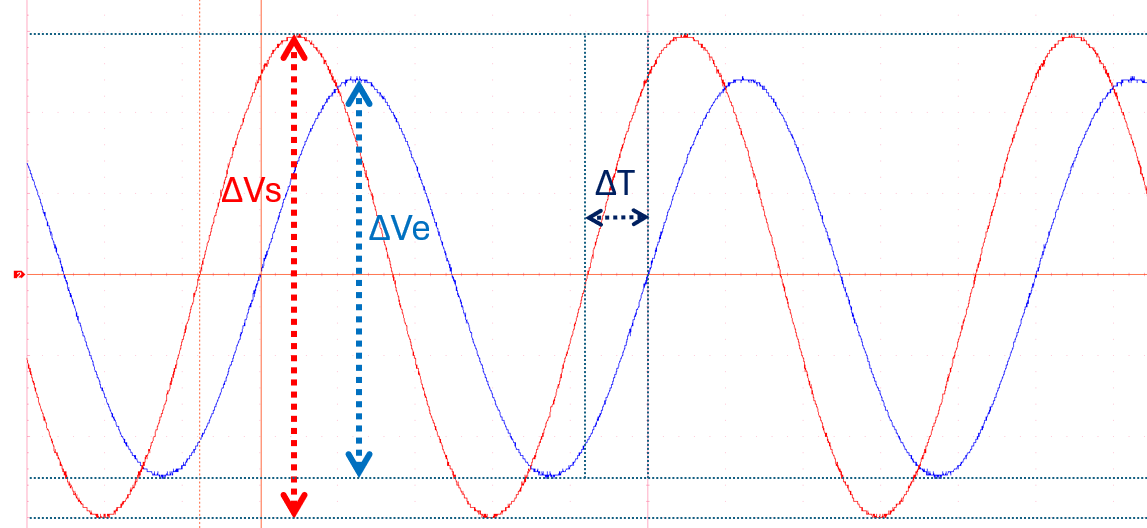
\includegraphics[width=0.8\textwidth]{images/rf_bode.png}
	
    \caption{Capture d'écran d'oscilloscope d'un signal sinusoïdal $V_E$ (en bleu) appliqué à un système linéaire et sa sortie $V_S$ (en rouge). Le calibre vertical est de 200mV/carreau pour $V_E$ et pour $V_S$. L'échelle horizontale est de 2ms/carreau.}
    \label{fig:rf_mesure}
\end{figure}

\newpage
\subsection{Mesure du gain du circuit}

Il existe \textbf{deux solutions pour déterminer la valeur du gain} :

\begin{itemize}
	\item Utiliser les mesures automatiques de l'oscilloscope, pour relever l'amplitude du signal d'entrée ($\Delta{}V_e$) et du signal de sortie ($\Delta{}V_s$), et utiliser un logiciel pour convertir le gain en $\operatorname{dB}$
	\item Utiliser le multimètre en dB-mètre (voir documentation annexe des instruments de mesure).
\end{itemize}

\medskip

On rappelle que le gain en décibel est égal à :

$$G_{dB} = 20 \cdot \log(A)$$

où $A = \frac{\Delta{}V_s}{\Delta{}V_e}$ est le gain du système.

\subsection{Mesure du déphasage}

Certains oscilloscopes proposent des mesures automatiques du déphasage. En leur absence, une mesure aux curseurs du décalage temporel $\Delta{}T$ entre les deux tensions (entrée et sortie) permet de remonter au déphasage $\Delta{}\phi$ par la formule :

$$\Delta{}\phi = +/- \frac{\Delta{}T}{T} \cdot 2\pi$$

où T est la période du signal.

Il est important de déterminer lequel des deux signaux est en avance sur l'autre, afin de donner un signe au déphasage apporté par le circuit. Si la tension de sortie est en retard sur la tension d'entrée, le déphasage est négatif.

\newpage
\section{Allure rapide}

Il existe également une \textbf{méthode automatique} pour obtenir l'allure de la réponse en fréquence du système, selon le modèle de GBF que vous possédez.

En effet, certains d'entre eux sont capables de réaliser automatiquement un balayage en fréquence.

Pour les GBF \textbf{\texttt{Agilent}} (des salles de TP d'électronique, par exemple), il faut utiliser au préalable sélectionner un \textbf{signal sinusoïdal}, de n'importe quelle fréquence mais d'amplitude et de valeur moyenne (offset) compatible avec le système à étudier (si ALI/AOP, vérifiez que le signal de sortie ne sature pas, par exemple).

Puis sélectionner ensuite le menu \textbf{Sweep} du GBF. Se référer ensuite à la documentation du GBF fournie sur vos paillasses pour les réglages (voir aussi figure~\ref{fig:gbf_sweep}).

\begin{figure}[h!]
    \centering
	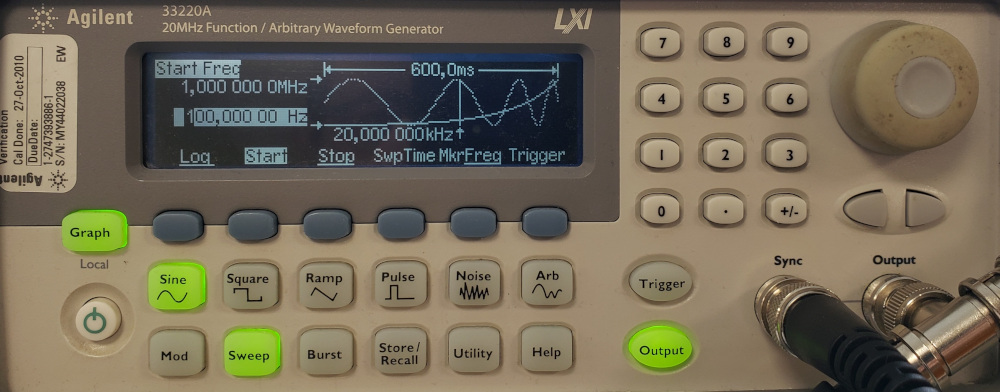
\includegraphics[width=0.6\textwidth]{images/gbf_sweep.jpg}
	
    \caption{Photographie d'un générateur de fonction Agilent 33220A en mode \textit{sweep} (balayage).}
    \label{fig:gbf_sweep}
\end{figure}


Il est ensuite possible de synchroniser l'oscilloscope avec le GBF en utilisant la sortie \textbf{Sync}, qui fournit un signal rectangulaire de même période que le balayage, connectée à l'une des entrées de l'oscilloscope (EXT si on ne souhaite que synchroniser) et en réglant les paramètres du déclenchement de l'oscilloscope.

\begin{figure}[h!]
    \centering
	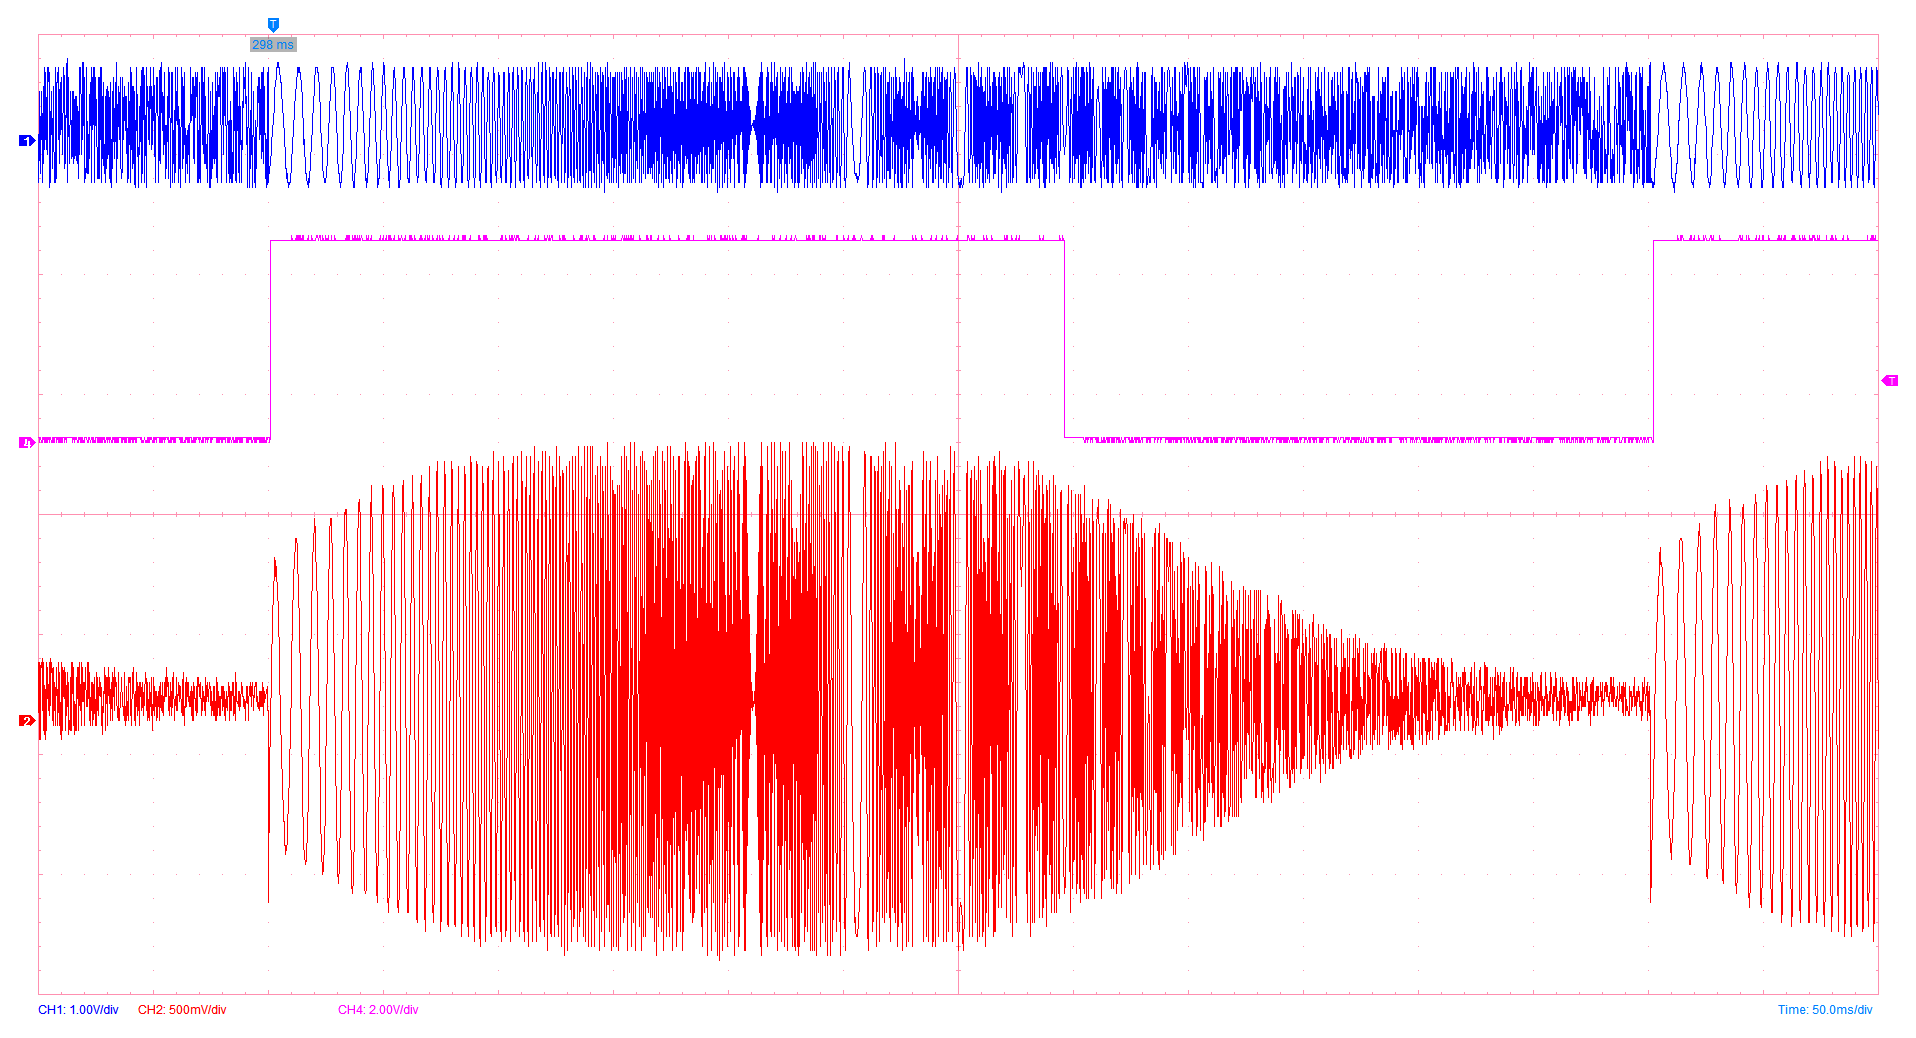
\includegraphics[width=0.7\textwidth]{images/gbf_sweep_sync.png}
	
	%Cas d'un passe-bande - en haut signal d'entrée (amplitude constante), au centre signal de synchronisation (avec marqueur en fréquence - retour à l'état bas) et en bas signal de sortie.

	
    \caption{Capture d'écran d'oscilloscope d'un balayage en fréquence $V_E$ (en bleu) appliqué à un système linéaire et sa sortie $V_S$ (en rouge) - cas d'un passe-bande. En haut signal d'entrée $V_E$ (amplitude constante), au centre signal de synchronisation (avec marqueur en fréquence - retour à l'état bas) et en bas signal de sortie $V_S$. Le calibre vertical est de 1V/carreau pour $V_E$ et de 200mV/carreau pour $V_S$. L'échelle horizontale est de 50ms/carreau.}
    \label{fig:rf_sweep}
\end{figure}

\newpage
\section{Quelques rappels}
%%%%%%%%%%%%%%%%%%%%%%%%%%%%%%%%%%
\subsection{Déphasage}

En régime harmonique (à même fréquence), deux ondes sinusoïdales peuvent avoir des phases initiales différentes.

Soient $u_1(t) = A_1 \cdot sin(2\pi f t + \varphi_1)$ et $u_2(t) = A_2 \cdot sin(2\pi f t + \varphi_2)$, le déphasage de l'une par rapport à l'autre à l'instant $t$ vaut : $\Delta\varphi = (2\pi f t + \varphi_2) - (2\pi f t + \varphi_1) = \varphi_2 - \varphi_1$

\medskip

Si $\Delta\varphi$ est positif, l'onde 2 est en avance de phase par rapport à l'onde 1. Sinon, l'onde 2 est en retard de phase par rapport à l'onde 1.

%%%%%%%%%%%%%%%%%%%%%%%%%%%%%%%%%%
\subsection{Phase et ordre d'un filtre}

Lorsqu'on étudie des systèmes linéaires de type filtre, il est intéressant de relever le déphasage entre le signal de sortie et le signal d'entrée pour différents points remarquables :

\begin{itemize}
	\item à la fréquence caractéristique du système, le déphasage est égal à $k\cdot \pi/4$ où $k$ est un entier correspondant à l'ordre du filtre
	\item loin de cette fréquence caractéristique (au moins une décade avant et après), pour vérifier le caractère inverseur d'un système par exemple.
\end{itemize}

\newpage
\pagestyle{empty}

\begin{minipage}[c]{.25\linewidth}
	
\includegraphics[width=4cm]{images/Logo-LEnsE.png}
\end{minipage} \hfill
\begin{minipage}[c]{.4\linewidth}

\begin{center}
\vspace{0.3cm}
{\Large \textsc{Opto-Electronique}}

\medskip

\textbf{\Large Ressources}

\end{center}
\end{minipage}\hfill

\vspace{0.5cm}

\noindent \rule{\linewidth}{1pt}
\section{Tracer la réponse en fréquence d'un système linéaire}
\label{ressource:RepFreq}


%%%%%%%%%%%%%%%%%%%%%%%%%%%%%%%%%%%%%%%%%%%%%%%%%%%%%%%%%%%%%%%%%%%%%%%%%%%%%%%%
%%%%%

La réponse en fréquence décrit la manière dont \textbf{un système réagit à différentes fréquences d'entrée}. Elle indique comment l'amplitude et la phase d'un signal sont modifiées lorsqu'il passe à travers un système ou un circuit, en fonction de la fréquence du signal.

Cette étude traduit le \textbf{comportement harmonique} d'un circuit, c'est à dire sa réponse à une excitation (en tension) sinusoïdale.

Cette fonction n'est définie que dans le cas de circuits linéaires. La tension de sortie est dans ce cas sinusoïdale et de même fréquence que le signal d'entrée.

\subsection{Objectif}

Obtenir l'allure de la \textbf{courbe du gain} et éventuellement de celle \textbf{du déphasage} apportés par le circuit en fonction de la fréquence du signal sinusoïdal placé en entrée.

Le \textbf{diagramme de Bode} est une manière spécifique de représenter la réponse en fréquence. Il s'agit d'une \textbf{représentation graphique} qui se compose de deux parties distinctes :

\begin{itemize}
	\item diagramme de Bode en gain (gain en $\operatorname{dB}$),
	\item diagramme de Bode en phase.
\end{itemize}

\bigskip

La courbe est souvent tracée avec une \textbf{échelle logarithmique} en fréquence. 

\subsection{Intérêt du passage en décibels (dB)}

Lorsqu'on cascade plusieurs systèmes entre eux, leurs fonctions de transfert se multiplient. Il n'est alors pas simple de pouvoir comparer \textbf{graphiquement} les systèmes à plusieurs étages facilement.

$$A = \prod_{k=1}^{n} A_k $$

En passant par une échelle logarithmique (en décibels par exemple), on transforme ce produit en une somme. Ainsi il sera plus simple de cumuler les effets d'une mise en cascade de systèmes linéaires et de voir le comportement global en additionnant les comportements de chacun des étages.

$$G_{dB} = \log(A) = \log(\prod_{k=1}^{n} A_k) = \sum_{k=1}^{n} \log(A_k) $$

\newpage
\subsection{Protocole d'étude}

\begin{itemize}
	\item Régler un \textbf{générateur de fonction} (ou GBF) pour avoir un \textbf{signal sinusoïdal} à sa sortie, avec une amplitude compatible avec les limites du circuit à tester.
	\item Relier le générateur de fonction à la fois à l'entrée du circuit et à une des entrées de l'oscilloscope.
	\item Relier la tension de sortie à une deuxième voie de l'oscilloscope.
	\item \textbf{S'assurer que le signal de sortie est bien sinusoïdal} avant d'aller plus loin. Dans le cas contraire, le système ne fonctionne pas de manière linéaire (amplitude trop élevée en entrée par exemple qui entraine une saturation en sortie...)
\end{itemize}


\section{Procédure classique}

Un premier balayage rapide en fréquence permet de \textbf{repérer les gammes de fréquences d'intérêt}.

Une analyse du \textbf{comportement du circuit pour les valeurs extrêmes de fréquences} (sur la phase et l'amplitude) apporte les informations sur le comportement asymptotique de la réponse en fréquence. Ce sont les \textbf{2 premiers points de mesure}.

\textbf{3 à 5 mesures supplémentaires} sont ensuite suffisantes :
\begin{itemize}
	\item l'une à la fréquence caractéristique du circuit, qui peut être : 
	\begin{itemize}
		\item la fréquence centrale d'un circuit passe-bande, 
		\item la bande passante à $-3\operatorname{dB}$ pour un circuit passe-bas ou passe-haut,
		\item la fréquence d'un déphasage particulier (en général la fréquence pour laquelle le déphasage apporté est égal à la moitié du déphasage maximal que le circuit peut apporter )
	\end{itemize}
	\item les autres de part et d'autres de cette fréquence caractéristique, à une octave au dessous (à la fréquence moitié) et une octave au dessus ( à la fréquence double)
\end{itemize}

\medskip

La figure~\ref{fig:rf_mesure} montre une capture d'écran d'oscilloscope d'un signal sinusoïdal $V_E$ appliqué à un système linéaire et sa sortie $V_S$. La méthode de mesure du gain du montage et du déphasage pour une fréquence particulière est représentée sur cette figure également.

\begin{figure}[h!]
    \centering
	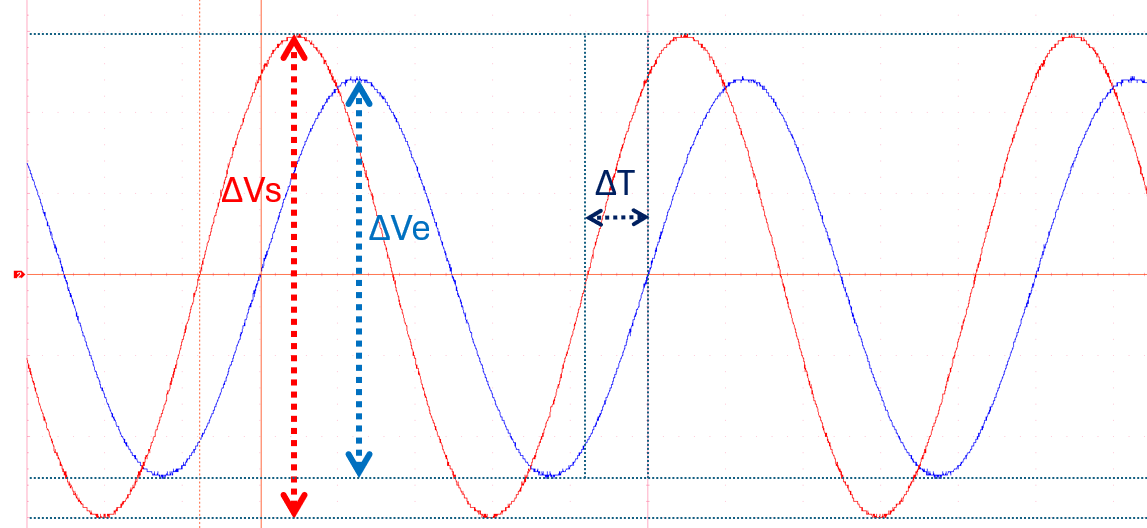
\includegraphics[width=0.8\textwidth]{images/rf_bode.png}
	
    \caption{Capture d'écran d'oscilloscope d'un signal sinusoïdal $V_E$ (en bleu) appliqué à un système linéaire et sa sortie $V_S$ (en rouge). Le calibre vertical est de 200mV/carreau pour $V_E$ et pour $V_S$. L'échelle horizontale est de 2ms/carreau.}
    \label{fig:rf_mesure}
\end{figure}

\newpage
\subsection{Mesure du gain du circuit}

Il existe \textbf{deux solutions pour déterminer la valeur du gain} :

\begin{itemize}
	\item Utiliser les mesures automatiques de l'oscilloscope, pour relever l'amplitude du signal d'entrée ($\Delta{}V_e$) et du signal de sortie ($\Delta{}V_s$), et utiliser un logiciel pour convertir le gain en $\operatorname{dB}$
	\item Utiliser le multimètre en dB-mètre (voir documentation annexe des instruments de mesure).
\end{itemize}

\medskip

On rappelle que le gain en décibel est égal à :

$$G_{dB} = 20 \cdot \log(A)$$

où $A = \frac{\Delta{}V_s}{\Delta{}V_e}$ est le gain du système.

\subsection{Mesure du déphasage}

Certains oscilloscopes proposent des mesures automatiques du déphasage. En leur absence, une mesure aux curseurs du décalage temporel $\Delta{}T$ entre les deux tensions (entrée et sortie) permet de remonter au déphasage $\Delta{}\phi$ par la formule :

$$\Delta{}\phi = +/- \frac{\Delta{}T}{T} \cdot 2\pi$$

où T est la période du signal.

Il est important de déterminer lequel des deux signaux est en avance sur l'autre, afin de donner un signe au déphasage apporté par le circuit. Si la tension de sortie est en retard sur la tension d'entrée, le déphasage est négatif.

\newpage
\section{Allure rapide}

Il existe également une \textbf{méthode automatique} pour obtenir l'allure de la réponse en fréquence du système, selon le modèle de GBF que vous possédez.

En effet, certains d'entre eux sont capables de réaliser automatiquement un balayage en fréquence.

Pour les GBF \textbf{\texttt{Agilent}} (des salles de TP d'électronique, par exemple), il faut utiliser au préalable sélectionner un \textbf{signal sinusoïdal}, de n'importe quelle fréquence mais d'amplitude et de valeur moyenne (offset) compatible avec le système à étudier (si ALI/AOP, vérifiez que le signal de sortie ne sature pas, par exemple).

Puis sélectionner ensuite le menu \textbf{Sweep} du GBF. Se référer ensuite à la documentation du GBF fournie sur vos paillasses pour les réglages (voir aussi figure~\ref{fig:gbf_sweep}).

\begin{figure}[h!]
    \centering
	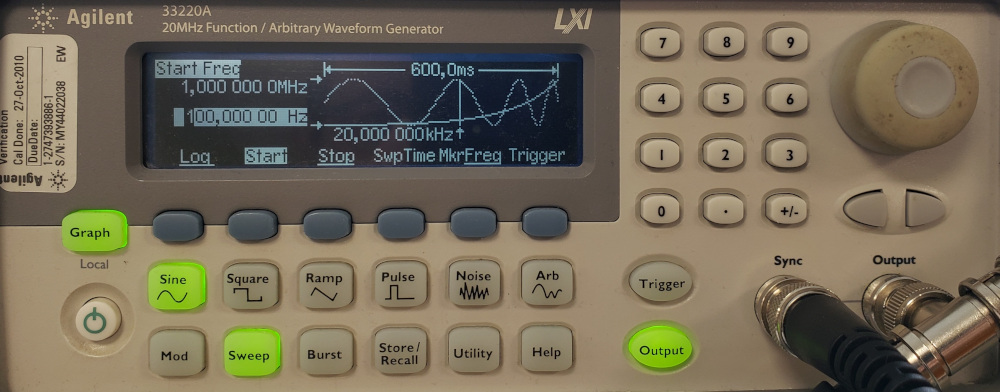
\includegraphics[width=0.6\textwidth]{images/gbf_sweep.jpg}
	
    \caption{Photographie d'un générateur de fonction Agilent 33220A en mode \textit{sweep} (balayage).}
    \label{fig:gbf_sweep}
\end{figure}


Il est ensuite possible de synchroniser l'oscilloscope avec le GBF en utilisant la sortie \textbf{Sync}, qui fournit un signal rectangulaire de même période que le balayage, connectée à l'une des entrées de l'oscilloscope (EXT si on ne souhaite que synchroniser) et en réglant les paramètres du déclenchement de l'oscilloscope.

\begin{figure}[h!]
    \centering
	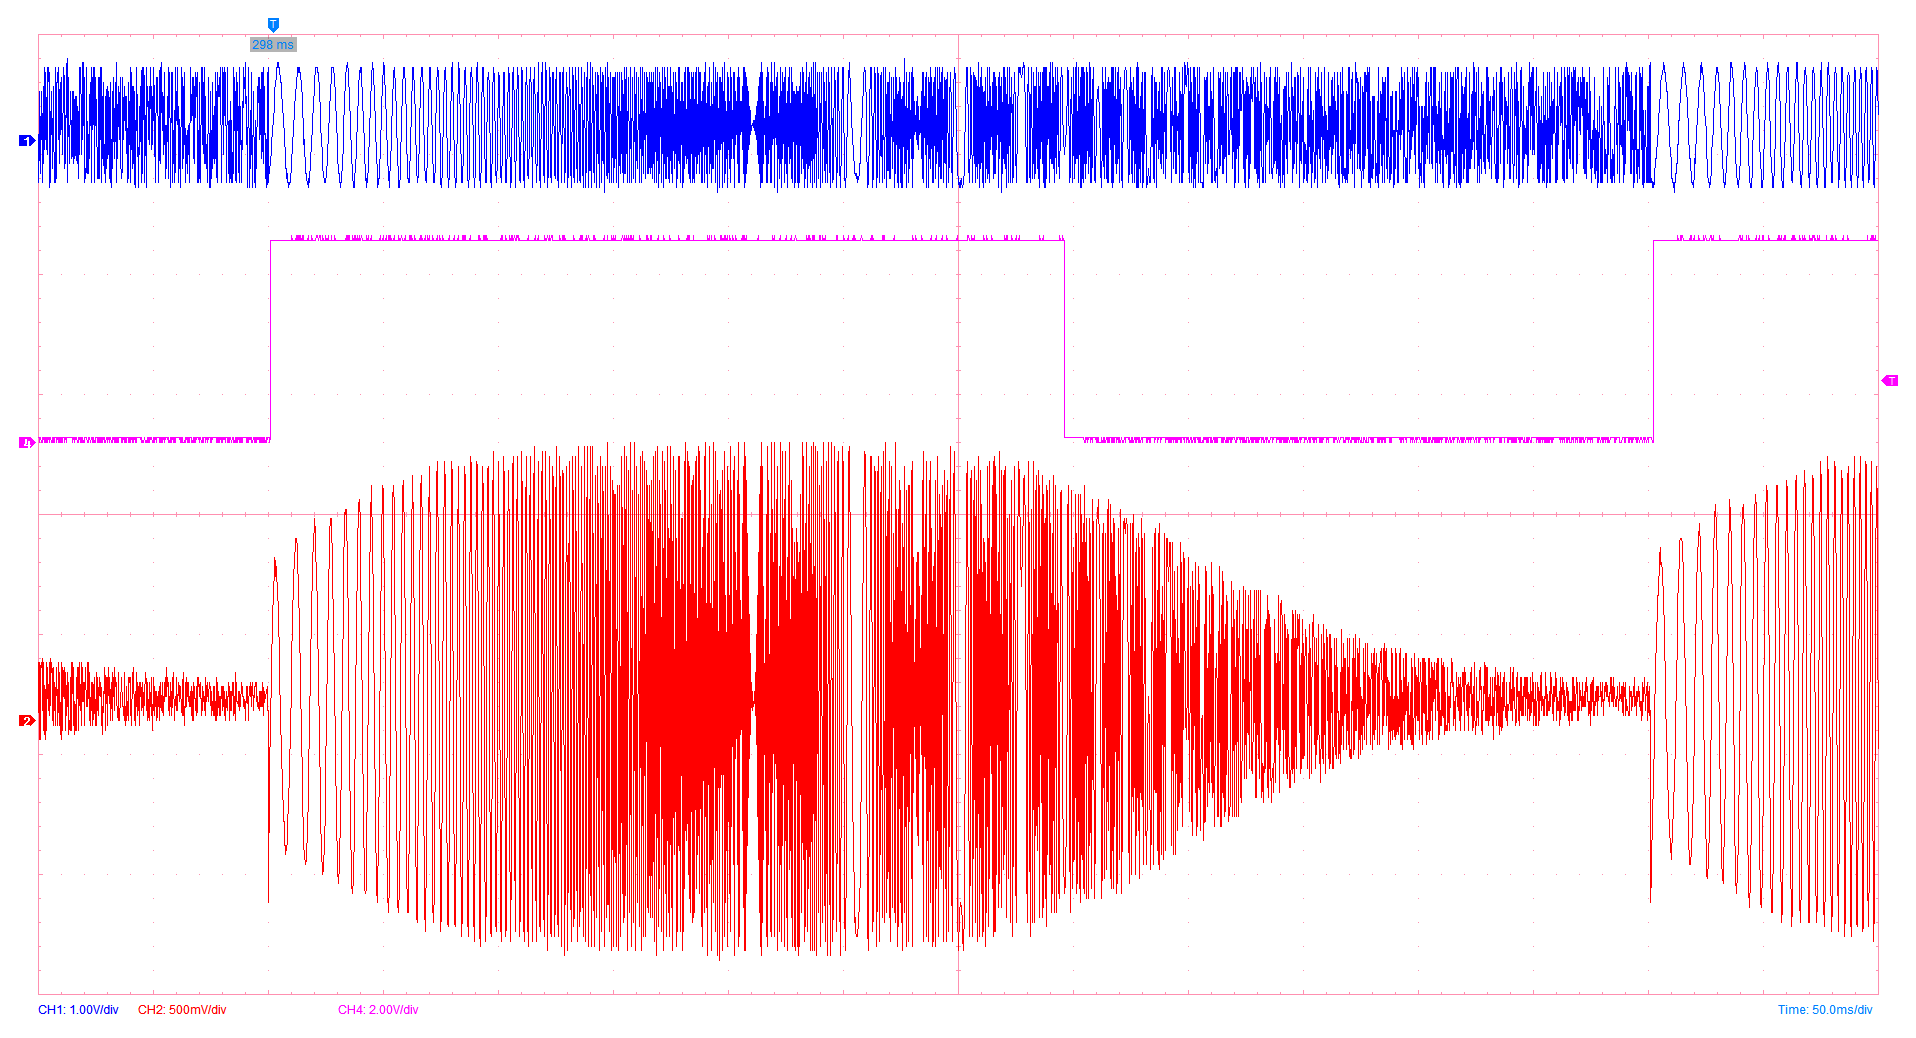
\includegraphics[width=0.7\textwidth]{images/gbf_sweep_sync.png}
	
	%Cas d'un passe-bande - en haut signal d'entrée (amplitude constante), au centre signal de synchronisation (avec marqueur en fréquence - retour à l'état bas) et en bas signal de sortie.

	
    \caption{Capture d'écran d'oscilloscope d'un balayage en fréquence $V_E$ (en bleu) appliqué à un système linéaire et sa sortie $V_S$ (en rouge) - cas d'un passe-bande. En haut signal d'entrée $V_E$ (amplitude constante), au centre signal de synchronisation (avec marqueur en fréquence - retour à l'état bas) et en bas signal de sortie $V_S$. Le calibre vertical est de 1V/carreau pour $V_E$ et de 200mV/carreau pour $V_S$. L'échelle horizontale est de 50ms/carreau.}
    \label{fig:rf_sweep}
\end{figure}

\newpage
\section{Quelques rappels}
%%%%%%%%%%%%%%%%%%%%%%%%%%%%%%%%%%
\subsection{Déphasage}

En régime harmonique (à même fréquence), deux ondes sinusoïdales peuvent avoir des phases initiales différentes.

Soient $u_1(t) = A_1 \cdot sin(2\pi f t + \varphi_1)$ et $u_2(t) = A_2 \cdot sin(2\pi f t + \varphi_2)$, le déphasage de l'une par rapport à l'autre à l'instant $t$ vaut : $\Delta\varphi = (2\pi f t + \varphi_2) - (2\pi f t + \varphi_1) = \varphi_2 - \varphi_1$

\medskip

Si $\Delta\varphi$ est positif, l'onde 2 est en avance de phase par rapport à l'onde 1. Sinon, l'onde 2 est en retard de phase par rapport à l'onde 1.

%%%%%%%%%%%%%%%%%%%%%%%%%%%%%%%%%%
\subsection{Phase et ordre d'un filtre}

Lorsqu'on étudie des systèmes linéaires de type filtre, il est intéressant de relever le déphasage entre le signal de sortie et le signal d'entrée pour différents points remarquables :

\begin{itemize}
	\item à la fréquence caractéristique du système, le déphasage est égal à $k\cdot \pi/4$ où $k$ est un entier correspondant à l'ordre du filtre
	\item loin de cette fréquence caractéristique (au moins une décade avant et après), pour vérifier le caractère inverseur d'un système par exemple.
\end{itemize}

\titleformat{\section}
  {\null}{}{0pt}{}

%% Docs techniques
%\includepdf[pages=4, pagecommand={\section{\texorpdfstring{\hspace{-1em}}{Doc SFH206K photodiode}}}\label{doc:phdSFH206K}]{ressources/osram_SFH206K.pdf}
%\includepdf[pages=5-8]{ressources/osram_SFH206K.pdf}



%% Fiches 
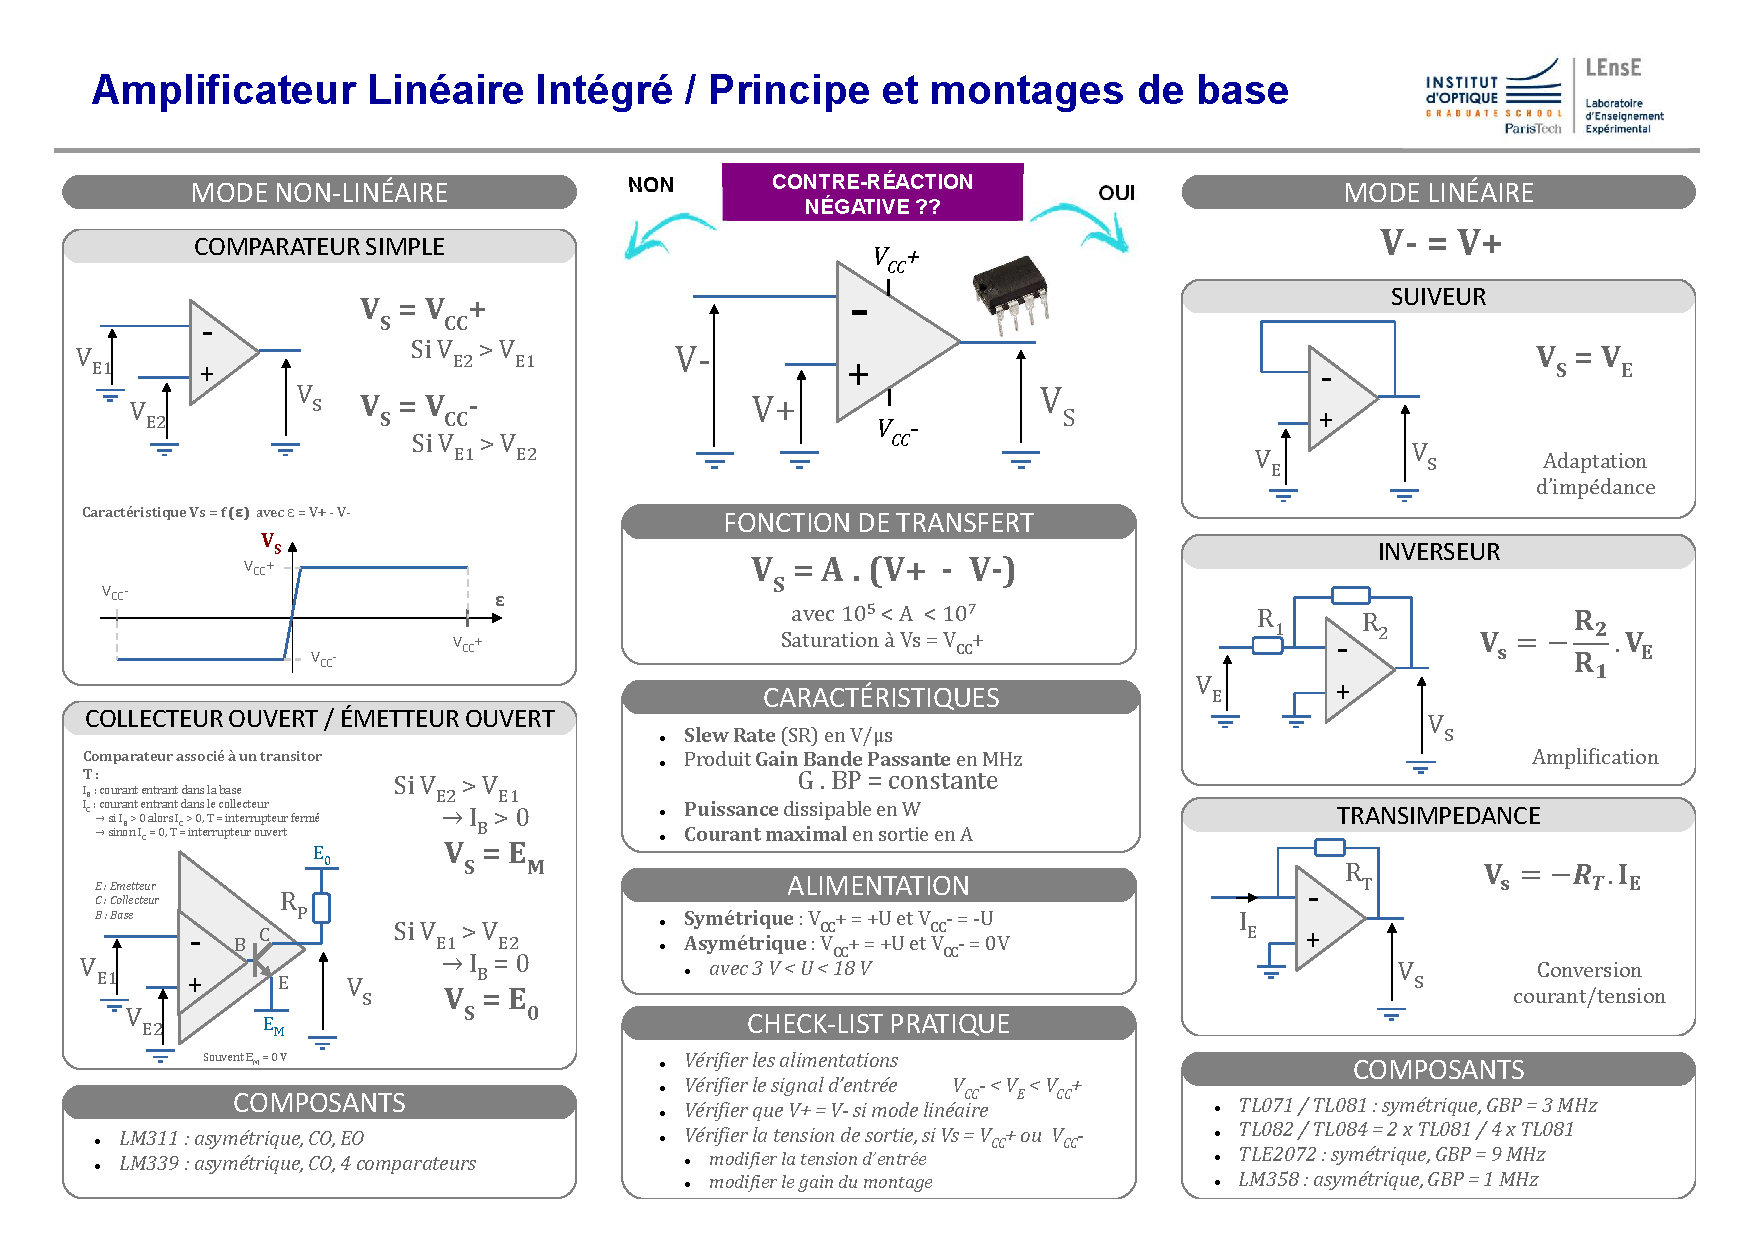
\includepdf[pages=-, landscape=true, pagecommand={\section{\texorpdfstring{\hspace{-1em}}{Fiche ALI}}}\label{fiche:ALI}]{../../Fiches/Fiche_ALI.pdf}

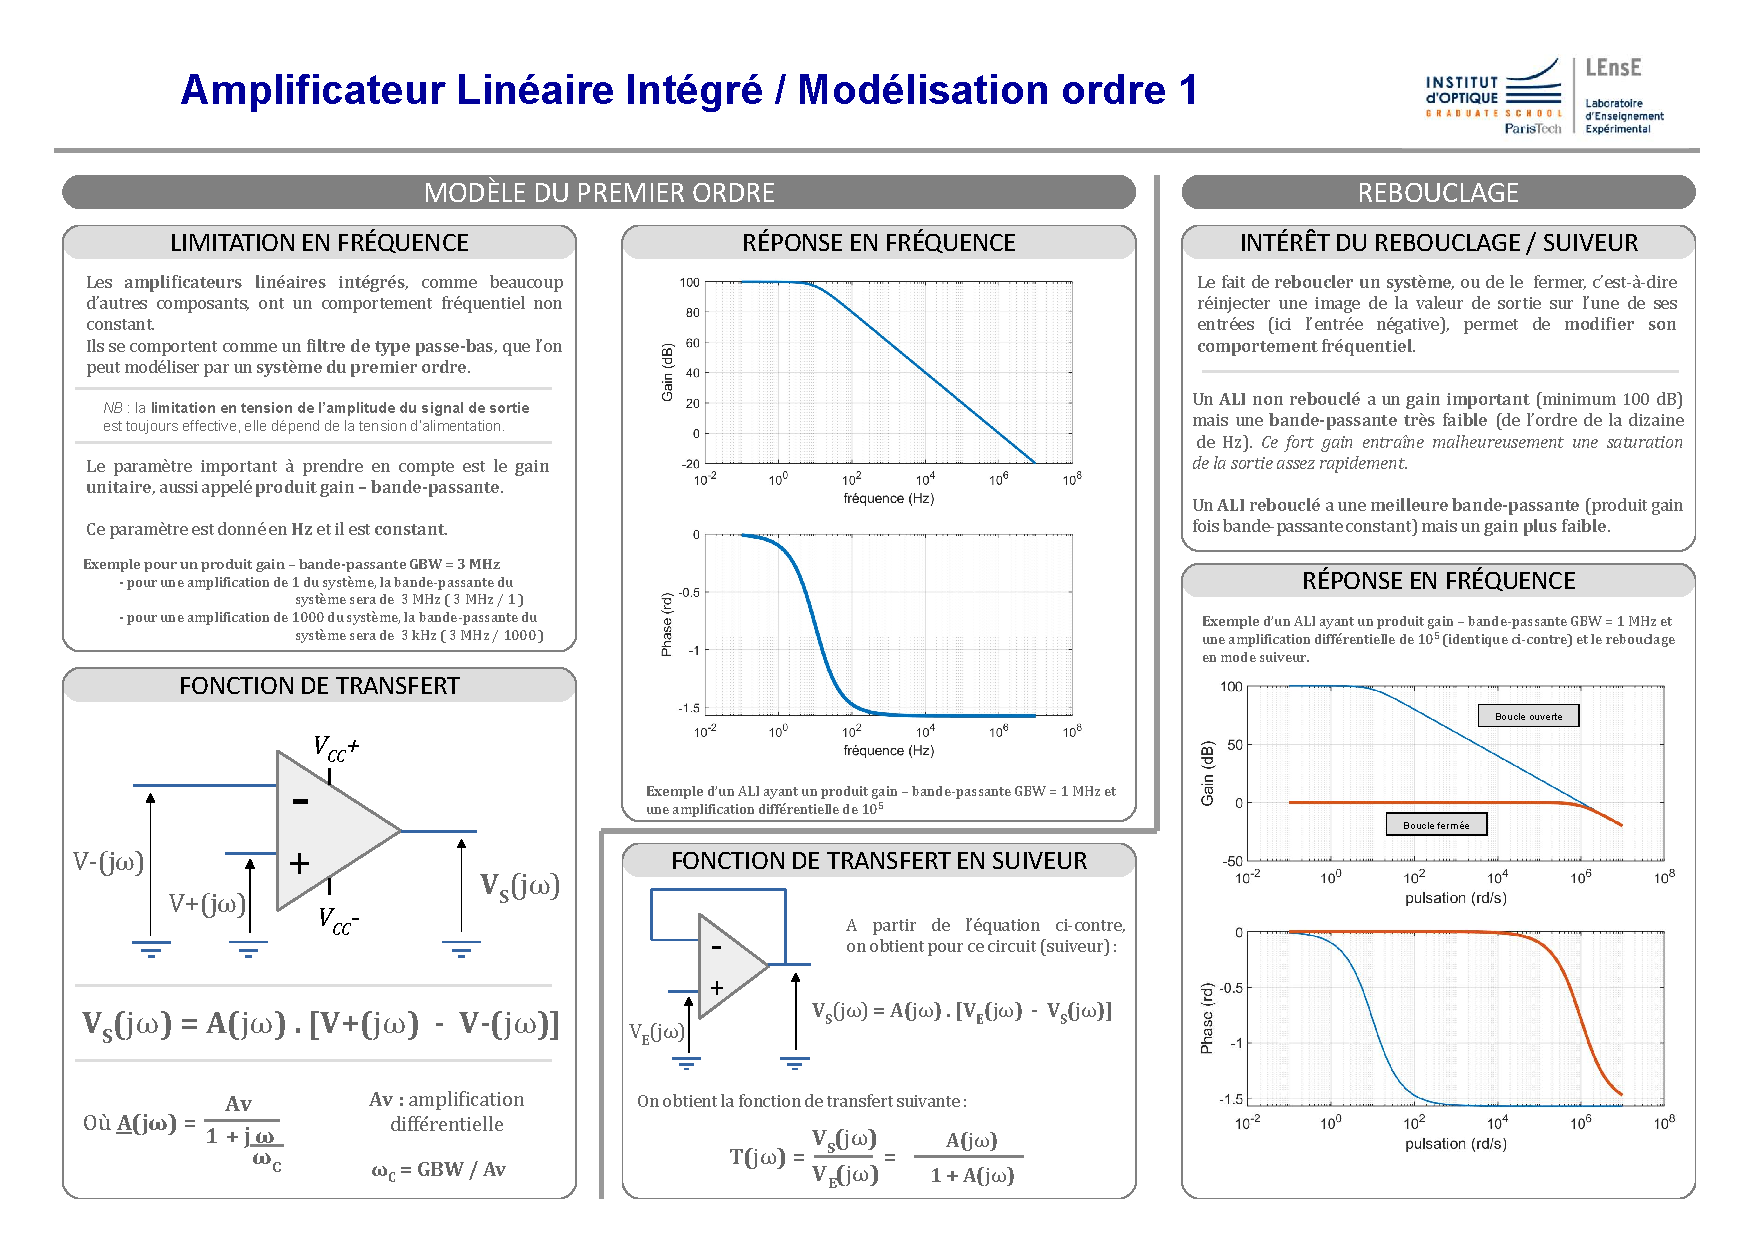
\includepdf[pages=-, landscape=true, pagecommand={\section{\texorpdfstring{\hspace{-1em}}{Fiche ALI Modele}}}\label{fiche:ALIModele}]{../../Fiches/Fiche_ALI_Modele.pdf}

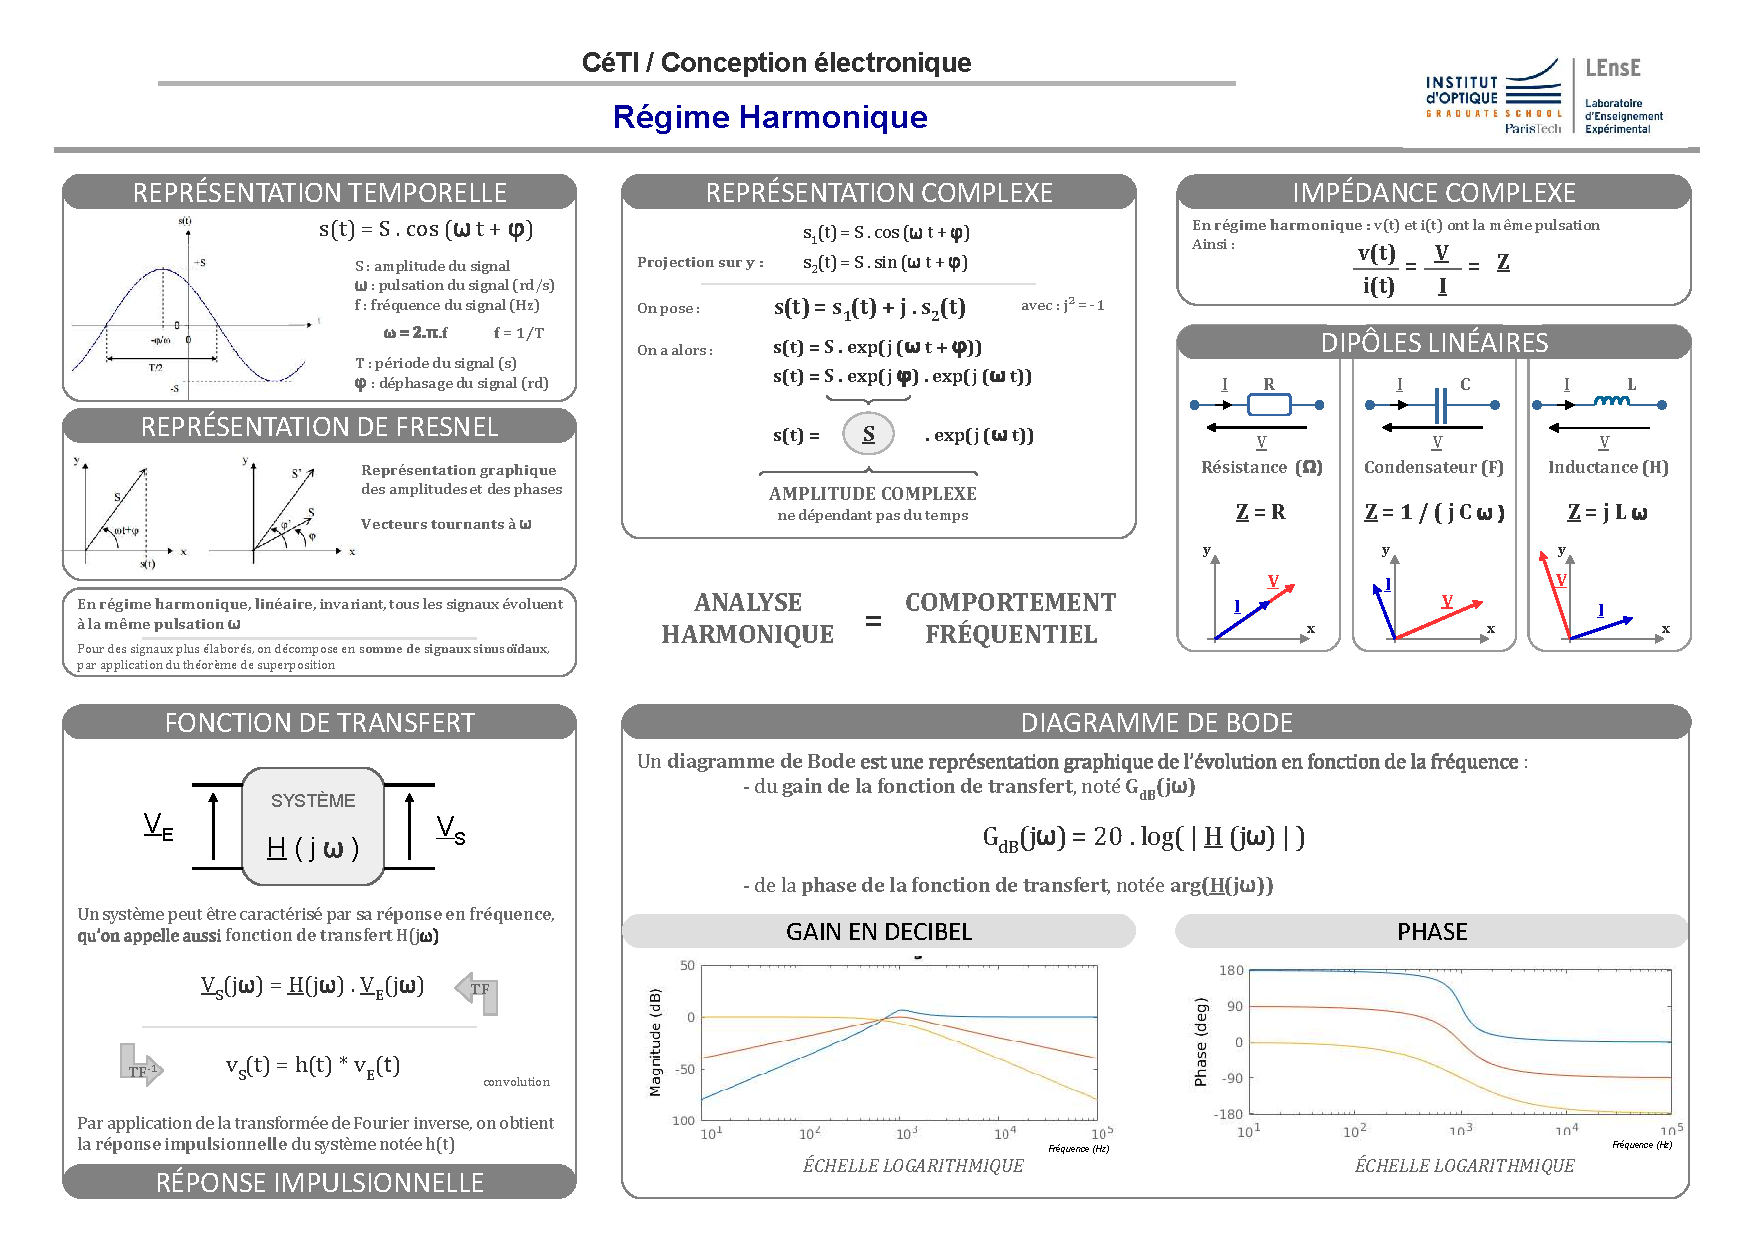
\includepdf[pages=-, landscape=true, pagecommand={\section{\texorpdfstring{\hspace{-1em}}{Fiche Regime Harmonique}}}\label{fiche:RegimeHarmonique}]{../../Fiches/Fiche_Regime_Harmonique.pdf}


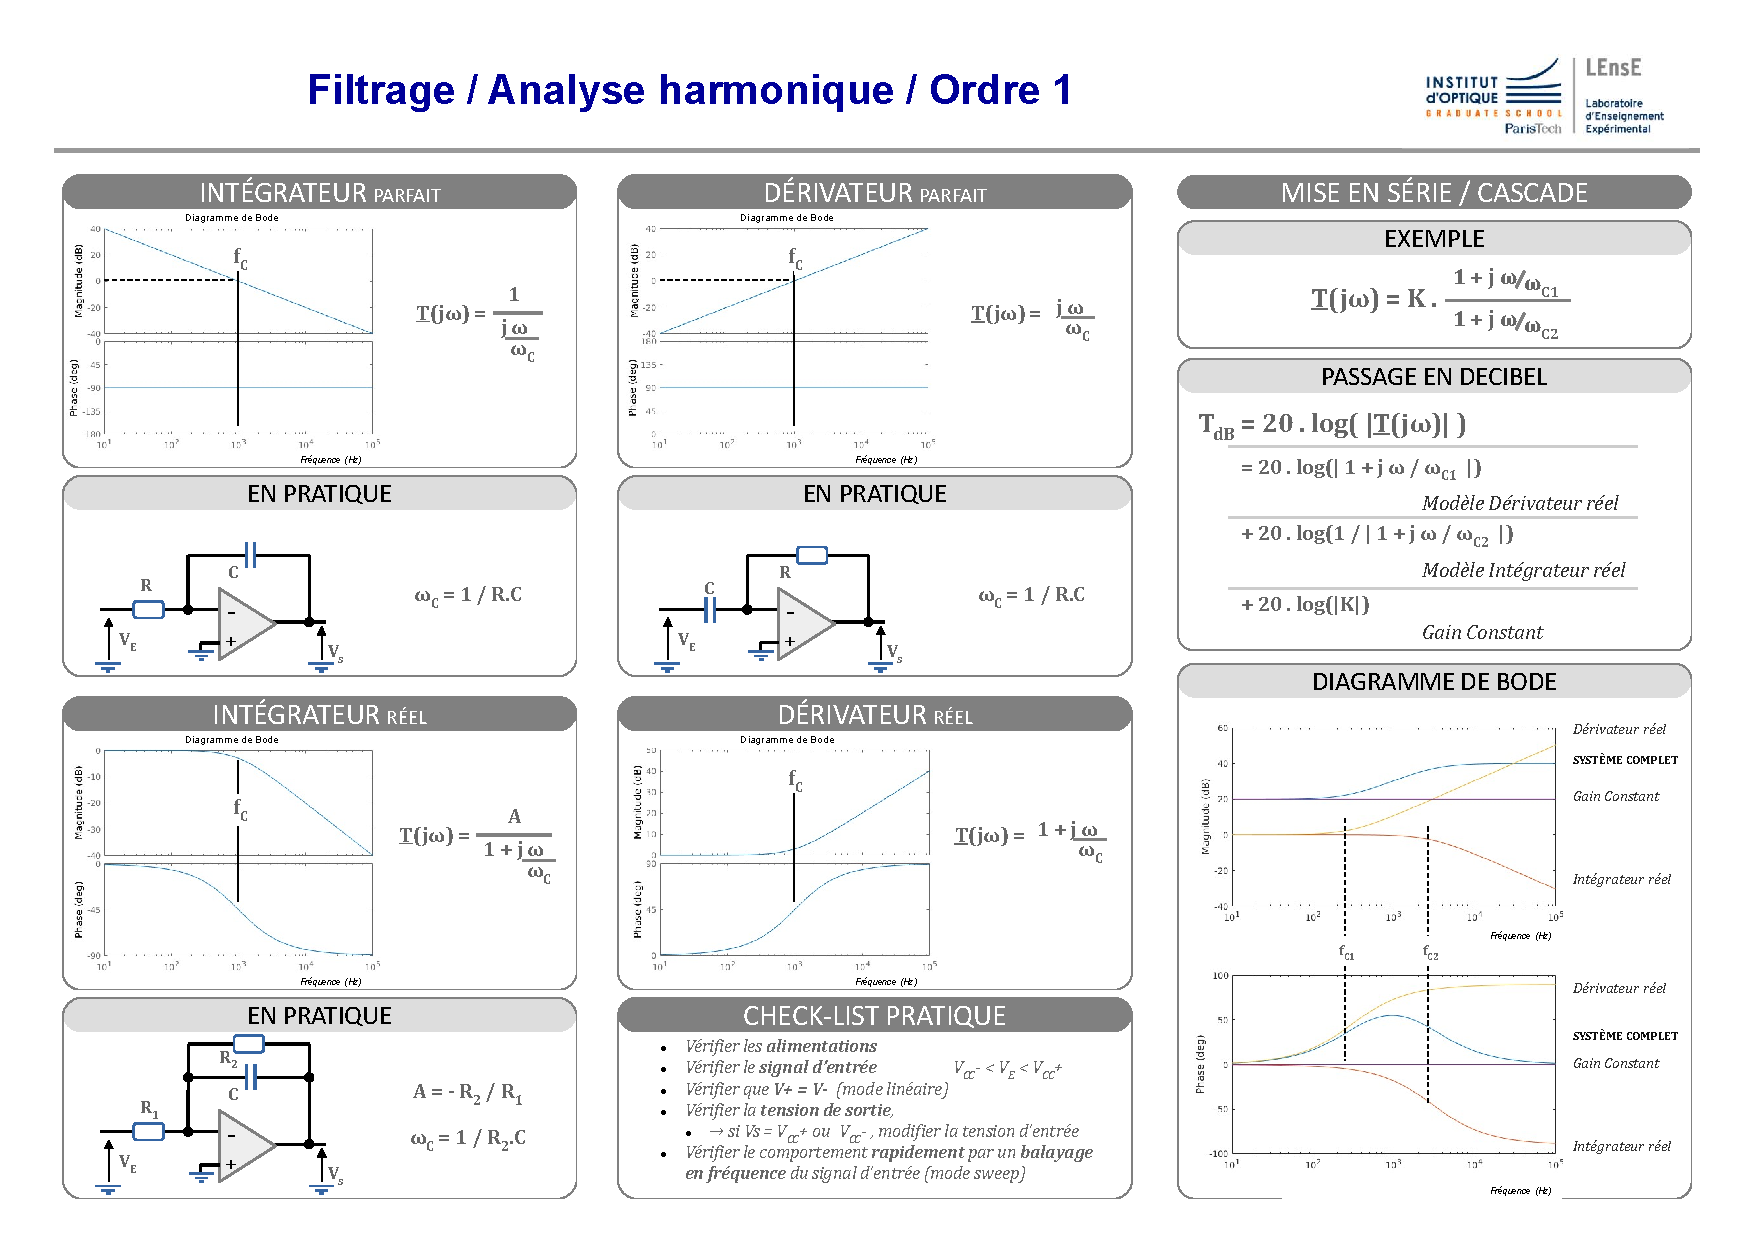
\includepdf[pages=-, landscape=true, pagecommand={\section{\texorpdfstring{\hspace{-1em}}{Fiche Analyse Harmonique Ordre 1}}}\label{fiche:AnHaOrdre1}]{../../Fiches/Fiche_Analyse_Ordre1.pdf}



\end{document}


